              
%++++++++++++++++++++++++++++++++++++++++
% Don't modify this section unless you know what you're doing!
\documentclass[a4paper,titlepage]{book}
\usepackage[italian]{babel}
\usepackage[T1]{fontenc}
\usepackage[utf8]{inputenc}
\usepackage[italian]{babel}
\usepackage{tabularx} % extra features for tabular environment
\usepackage{verbatim}
\usepackage{fancyhdr}
\usepackage{tocbibind}
\newenvironment{abstract}%
{\cleardoublepage%
	\thispagestyle{empty}%
	\null \vfill\begin{center}%
		\bfseries \abstractname \end{center}}%
{\vfill\null}
\usepackage{siunitx}
\usepackage[swapnames]{frontespizio}
\usepackage{amsmath}  % improve math presentation
\usepackage{graphicx} % takes care of graphic including machinery
\usepackage[bottom=2cm]{geometry} % decreases margins
\usepackage{cite} % takes care of citations
\usepackage[final]{hyperref} % adds hyper links inside the generated pdf file
\hypersetup{
    colorlinks=true,       % false: boxed links; true: colored links
    linkcolor=blue,        % color of internal links
    citecolor=blue,        % color of links to bibliography
    filecolor=magenta,     % color of file links
    urlcolor=blue      
}
%++++++++++++++++++++++++++++++++++++++++


\begin{document}
	
	\begin{frontespizio}
	\begin{Preambolo*}
		\usepackage{fourier}
		\newcommand{\VOF}{\textsc{vof}}
	\end{Preambolo*}
		\Universita{Perugia}
		\Logo[3cm]{Logo-Universit-degli-Studi-di-Perugia.jpg}
		\Facolta{Fisica}
		\Corso[Laurea]{Triennale in Fisica L30}
		\Titoletto{Tesi di laurea}
		\Titolo{Studio sulle forme allotropiche del Carbonio}
		\Candidato[282162]{Arianna Mischianti}
		\Relatore{Prof.~Andrea Orecchini}
		\Annoaccademico{2018-2019}
	\end{frontespizio}

\null\vspace{\stretch{1}}
\begin{flushright}
	\textit{Ai miei genitori}
\end{flushright}
\vspace{\stretch{2}}\null
\newpage

\begin{abstract}
	Il presente lavoro è volto ad eseguire una rassegna degli allotropi del carbonio. Si classificano e si evidenziano caratteristiche, proprietà fisiche, sintetizzazione e scoperta, ed eventuali applicazioni possibili. Ci si sofferma maggiormente su uno studio del reticolo cristallino, riportando anche la dispersione fononica.\\
	
	
	\textit{As described by Smalley, the formation of a fullerene follows an "efficient mechanism of self-assembly of an architecturally useful structure on a nanometer scale."} 
\end{abstract}

\tableofcontents
\chapter{Introduzione}

\section{Generalità sul carbonio}

Il Carbonio (dal latino "carbo", ossia carbone) è un elemento chimico conosciuto fin dall'era preistorica. La scoperta del carbonio ha rivoluzionato la scienza e la tecnologia di ieri, oggi e domani: si crede che lo sviluppo di materiali contenenti carbonio sarà cruciale per il futuro della chimica e la tecnologia; l'avvenire della nanotecnologia e la nanoscienza è anche collegato al largo impiego di carbonio per la fabbricazione di componenti. In fase solida presenta varie forme allotropiche, il che lo rende un elemento incredibilmente versatile, e risulta ampiamente distribuito in natura: lo ritroviamo nelle molecole organiche, ma anche in ambienti extraterrestri e nella materia del cosmo. Detiene il sesto posto nella lista delle abbondanze dell'universo, mentre nel corpo umano la presenza del carbonio è seconda solo a quella dell'ossigeno. Il suo ruolo nei meccanismi naturali è determinante: si basti pensare al fatto che il meccanismo biochimico (responsabile della vita) è di fatto altamente dipendente dal ruolo del carbonio sia direttamente che indirettamente. Il carbonio è infatti l'unico elemento ad essere presente in tutte le molecole organiche, caratterizzandone l'attitudine a stabilire legami e a dare forma a strutture molecolari complesse.
Il carbonio esiste in natura in due forme isotopiche: $^{12} C$ molto più abbondante, e $^{13} C$. Il nucleo del carbonio $^{12}C$ è composto da sei protoni e sei neutroni. Il carbonio neutro ha configurazione allo stato fondamentale  $1s^22s^22p^2$; è tetravalente e dispone di 6 elettroni, dei quali quattro di loro occupano l'orbita più esterna $2s^22p^2$ .

\section{Legami che forma} \label{legami}
Il carbonio forma legami covalenti attraverso un'ibridazione degli orbitali.
\begin{figure}[h] 
	\centering 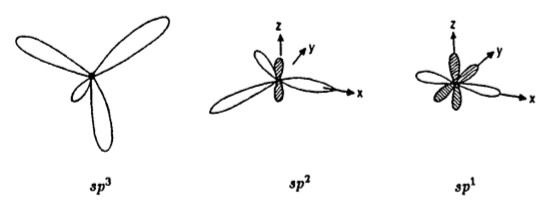
\includegraphics[width=1\columnwidth]{bondings.png}
	\caption{
		\label{fig:bond}  rappresentazione schematica dei legami ibridi $sp$, $sp^2$, $sp^3$. Gli spazi vuoti indicano legami forti, gli spazi riempiti indicano legami deboli.
	}
	\label{fig:bonds}
\end{figure}

I legami che forma dipendono dalla fase solida interessata. Le fasi allotropiche monodimensionali sono formate da legami ibridi di tipo $sp$, ossia quando un orbitale $s$ si svrappone ad un orbitale di tipo $p$. I 2 orbitali ibridi ottenuti si dispongono lungo un asse con un angolo di $180^\circ$, gli orbitali $p$ non ibridati, contenenti gli elettroni non legati, si dispongono perpendicolari tra loro, ed il piano formato risulta perpendicolare agli orbitali ibridi (figura \ref{fig:bond}). Quando ad esempio il carbonio solidifica in grafite i legami che si formano con i tre primi vicini (provenienti dagli orbitali $2s$, $2p_x$, e $2p_y$) sono tre legami forti complanari formanti angoli di $120^\circ$, l'orbitale p non ibridato si pone perpendicolarmente agli altri 3; quest'arrangiamento di legami è chiamato $sp^2$. Gli elettroni rimanenti che si trovano nell'orbitale  $p_z$ contribuiscono solo ai legami deboli interplanari, ma sono i responsabili del comportamento semimetallico della grafite. Nella struttura del diamante i legami che coinvolgono un carbonio ed i suoi quattro primi vicini, sono tetraedrici e sono composti dalla combinazione lineare di $2s$, $2p_x$, $2p_y$, e $2p_z$ formando angoli di $109.5^\circ$, essendo una configurazione del tipo $sp^3$. La differenza strutturale delle forme allotropiche del carbonio da vita alla diversificazione delle loro proprietà fisiche.

\section{Forme allotropiche}


Nel 1772, Antoine Lavoisier comprese che il carbonio disponeva di almeno due forme allotropiche grazie al famoso esperimento nel quale scoprì che bruciando un campione di diamante e uno di carbone con stessa massa si produce la stessa quantità di $CO_2$, dunque concluse che sono formate dallo stesso elemento, il carbonio. Ad oggi sappiamo che \textit{il diamante, la grafite, i fullereni, il carbonio acetilenico lineare, i nanotubi di carbonio, la nanoschiuma di carbonio} ed \textit{il carbonio amorfo} sono anch'esse forme allotropiche. Vi sono poi altre forme simili al diamante (\textit{lonsdaleite}). Le forme allotropiche più recenti sono \textit{la Q-Carbon(2015), T-Carbon(2011),D-Carbon(2018) , il novamene(2017), ed il protomene(2018)}.

\section {Diagramma di fase}

In accordo con il diagramma di fase, la grafite, il diamante, la fase liquida e di vapore del carbonio sono forme termodinamicamente stabili.
In condizioni standard (temperature $25^\circ$  celsius e pressione $1 atm$) si ha il carbonio in fase di grafite, come indicato dal diagramma di fase in figura. Se si applicano pressioni elevate ed alte temperature (nel caso di processo di catalisi con metallo liquido, utilizzando ferro o nichel, entrambe portate a $2000 K$ e $6-10 GPa$ ) avviene la trasformazione della grafite in diamante. Una volta diminuita la pressione, il diamate rimane stabile sebbene sia in condizioni standard: esso è una fase metastabile del carbonio in condizioni standard, in quanto fondamentalmente il processo di ritrasformazione in grafite risulta essere un decadimento veramente molto lento. Se il diamante viene perturbato, come ad esempio esponendolo a irradiazione o calore, esso torna velocemente allo stadio di equilibrio a temperatura e pressione standard, ovvero la grafite; è necessaria dunque una determinata energia di attivazione.
Per sintetizzare il diamante dalla forma liquida invece servono temperature e pressioni anche più alte.
\begin{figure}[h] 
	\centering 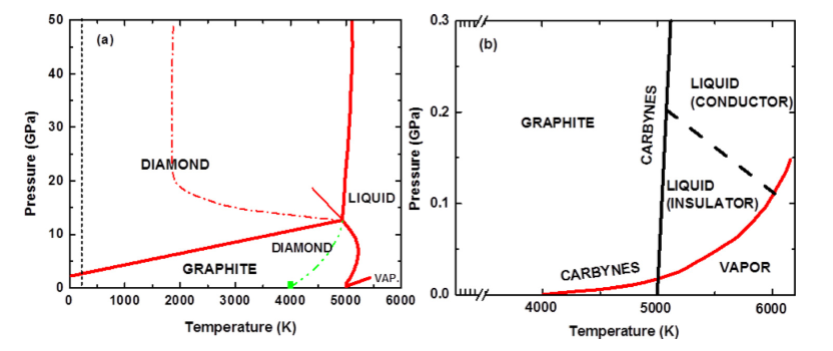
\includegraphics[width=1\columnwidth]{dyagramphase.png}
	\caption{
		\label{fig:dyagramphase}  $(a)$: diagramma di fase del carbonio $(P - T)$. $(b)$: diagramma di fase per basse pressioni e temperature.
	}
	\label{phases}
\end{figure}

A basse pressioni e temperature di circa $4000 K$ invece, la grafite è in grado di convertirsi in vapore. 
Il punto triplo di grafite/diamante/carbonio liquido si ottiene a $T=5000K$ e $P=12GPa$, dove $1GPa=9869atm$.
Dunque il diamante può esistere solo all'interno dei pianeti più distanti (Urano e Nettuno) e sul mantello della terra, dove la pressione-temperatura è di  $600 GPa-7000 K$ e $135 GPa-3500 K$, rispettivamente.
A causa dell'elevata energia di attivazione ed energia di legame necessaria per la trasformazione, il carbonio può esistere in più forme nella stessa regione $P-T$. 
La compressione a temperatura ambiente della grafite sviluppa il legame $sp^3$ a circa $12-14 GPa$, che porta alla diminuizione della conducibiltà elettrica e all'aumento della trasmittanza grazie alla rimozione degli elettroni di conduzione. La trasformazione è reversibile decomprimendo il sistema, tuttavia risulta irreversibile a pressioni e temperature ancora più elevate, in questo modo si crea il diamante esagonale, o lonsdaleite. 

\section {Criterio di suddivisione}
Di seguito si presenta il criterio di suddivisione del seguente resoconto di forme allotropiche ad oggi scoperte e sintetizzate. In base al tipo di legame ibrido che gli atomi di carbonio formano di cui si è parlato nel capitolo~\ref{legami}; di seguito dunque si riporta il suddetto criterio 
\begin{table}[ht]
	\begin{center}
		\caption{Criterio di suddivisione delle varie forme allotropiche.}
		
		\label{tab:crit} % spaces are big no-no withing labels
		\begin{tabular}{|c|c|} 
			\hline
			\multicolumn{1}{|c|}{Legame Ibrido} & \multicolumn{1}{c|}{Forma allotropica} \\
			\hline
			$sp$  &   \textit{Catena lineare di carbonio} \\
			$sp^2$ &  \textit{Grafite, grafene} \\
			$sp^3$ &    \textit{Diamante, lonsdaleite}\\
			$mixed \: sp^3/sp^2 \: forms$ &    \textit{Fullereni, nanotubi di carbonio, carbonio amorfo, nanoschiuma di carbonio}\\
			\hline
			\textit{le nuove fasi} &\textit{Q-Carbon, T-Carbon, novamene, protomene, D-Carbon} \\ %spazio fra le formule si fa così \: 
			\hline
		\end{tabular}
	\end{center}
\end{table}
in tabella \ref{tab:crit}. \\
Per ogni tipo di legame ibrido, qualora vi fossero più di una forma allotropica, si è scelto di procedere per ordine in base alla cronologia di scoperta.
\chapter{Carbonio acetilenico lineare}
\section{Scoperta e sintetizzazione}
Il carbonio acetilenico lineare o carbina (in inglese carbynes, linear acetylenic carbon) è stato oggetto di ricerca per tanti anni. Esso consiste in catene di carbonio del tipo\\
\begin{equation}
	\dots C-C-C \dots per \: n>10\\
\end{equation} 
sottoposte al processo di tempra. Questa struttura è stabile a modeste pressioni e temperature comprese fra $2700 K< T < 4500 K$. (come si vede nel diagramma di fase in fig. \ref{phases}). Si presenta di colore bianco-argenteo e lo troviamo nei campioni di meteoriti, dove le carbine si trovano mescolate alle particelle di grafite. Furono identificate per la prima volta in campioni trovati nel cratere di Nördlingen in Baviera. Inoltre, si è in grado di riprodurle in laboratorio attraverso quattro processi differenti: la sublimazione della grafite pirolitica per mezzo della tecnologia ad alto vuoto, la deidrogenazione dell'acetilene, la scomposizione di composti organici,e anche grazie ad un rapido processo di solidificazione del carbonio liquido.  


\section {Reticolo cristallino}
\subsection{Struttura del reticolo}
La sua struttura cristallina è stata studiata con il metodo della diffrazione a raggi X attraverso l'identificazione dei picchi di Bragg, utilizzando le carbine sintetiche prodotte dalla sublimazione della grafite pirolitica. 
Sulla base dei dati ricavati dalla distribuzione di densità elettronica si è prodotto un modello per il reticolo cristallino delle carbine che mostrava una struttura alternata, come se fosse costituito da due strati periodici. Secondo questo modello, rappresentato in fig. \ref{cri}, la cella unitaria delle carbine è costituita da catene di carbonio tenute insieme dalle forze di van-der-Waals, ottenendo così una struttura a doppio strato. Nello strato inferiore le catene sono strettamente collegate e posizionate agli angoli (1 e 2) e al centro (3) di un esagono, mentre nello strato superiore manca la catena centrale che troviamo nel primo strato, formando un vuoto dove possono prendere posizione degli atomi di impurità (fig. \ref{cri}).\\ 
\begin{figure}[h] 
	\centering 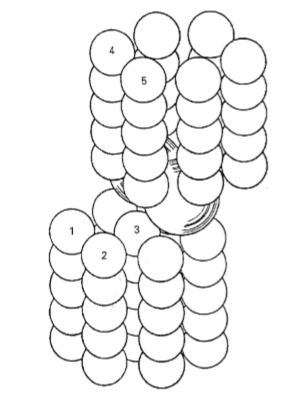
\includegraphics[width=0.4\columnwidth]{carbynecrystal.png}
	\caption{
		Reticolo cristallino delle carbine.
	}
	\label{cri}
\end{figure}
Vi sono differenti tipi di carbine, di cui ne sono state identificate almeno due. Hanno rispettivamente parametri di reticolo $a_\alpha= \SI{ 8.94}{\angstrom}$ e $c_\alpha =  \SI{ 15.36}{\angstrom}$; mentre $a_\beta =  \SI{ 8.24}{\angstrom}$  e  $c_\beta= \SI{ 7.68}{\angstrom}$. Applicando una pressione sul tipo $\alpha$ si ottiene il tipo $\beta$. Il numero di atomi per cella unitaria e la densità sono rispettivamente $\eta=144$ e  $\rho=2.68\, g/cm^3$ per la fase $\alpha$ e  di $\eta=72$ e $\rho=3.13\, g/cm^3$ per la fase $\beta$.
\subsection{Dispersione fononica}
Per quello che concerne la dispersione fononica delle carbine invece, in un lavoro di Milani et al. \cite{phono} si è trovato il diagramma \ref{fig:ccc} che mostra i rami di dispersione fononica  ottenuti attraverso due metodologie differenti che utilizzano la teoria del funzionale di densità (Density Functional Theory, DFT), ossia una teoria quantistica microscopica per lo studio di sistemi a molti elettroni).
\begin{figure}[h!] 
	\centering 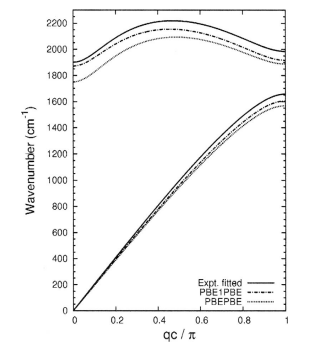
\includegraphics[width=0.6\columnwidth]{phocarb.png}
	\caption{
		Rami longitudinali di dispersione fononica.Nel calcolo dei rami sono state considerate le interazioni fino al 40esimo vicino.
	}
	\label{fig:ccc}
\end{figure}

I rami di dispersione di fononi ottenuti danno risultati rilevanti: il ramo longitudinale ottico si trova nell'intervallo $1900-2200 cm^{-1}$; le loro frequenze sono fortemente modulate dal grado di delocalizzazione dell'elettrone. Le frequenze trovate attraverso approcci differenti del ramo LO mostrate in figura, sono in ottimo accordo con la curva che ci si aspettava dai calcoli. 
\section{Proprietà fisiche}
A causa della difficoltà nell'isolare le carbine si conosce molto poco delle loro proprietà fisiche.
Si comportano come un semiconduttore con un gap di $1-2 eV$. In fase solida presentano durezza intermedia fra diamante e grafite. La  capacità termica supera quella della grafite per un fattore di 1,5 a $T=80 K$ e la funzione $\sigma(T)$ segue una legge lineare, mentre quella della grafite e del diamante è conforme a una legge di potenza.
Nell'esperimento condotto da S. Kotrechko et al. \cite{Kotr}  si calcolò ad esempio il carico di rottura di una catena lineare.  
Il campione di carbine si ottenne attraverso l'utilizzo di un unico strato di grafene e di un campo elettrico: sotto l'influenza delle forze meccaniche del campo elettrico, le catene lineari si formano rompendo i legami della superficie del foglio di grafene
\begin{figure}[h!] 
\centering
 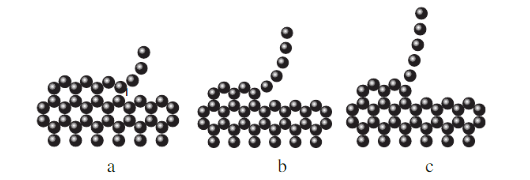
\includegraphics[width=0.8\columnwidth]{carbyne.png}
	\caption{ 	\label{cacca}
		Sintetizzazione delle catene di carbonio lineari da un foglio di grafene. Si riportano le fasi successive alla rottura dei legami del grafene sotto l'influenza di un campo elettrico, che produce un una forza di $7.82\: nN$, con conseguente allungamento della catena. Vengono visualizzate le configurazioni al momento iniziale \textit{(a)} e dopo un tempo $t=6.4\cdot10^{-14}s$  immagine \textit{(b)} e dopo un tempo $t=9.6\cdot10^{-14}s$ immagine \textit{(c)}.
	}
	\end{figure}
(figura \ref{cacca}).\\
 Una catena lineare contenente cinque atomi, ha un carico $F_c = 13,09 nN$. Aumentando il numero di atomi nelle catene si ha un aumento della rigidità della catena, e quindi del suo coefficiente di elasticità. Da $N>12$ in poi, la forza diventa indipendente dalla lunghezza della catena e raggiunge $F_c=12,35 nN$.  La stima sperimentale del suo stress critico è di $P=270 \,GPa \: (a\: T=5 K)$ e $P=251\, GPa \:(a \:T=77 K)$. è oltre due volte superiore allo stress critico del grafene $(P=130 \,GPa)$, il che lo rende uno dei materiali più resistenti al mondo.
 
 \section{applicazioni possibili}
Dalle carbine si possono produrre materiali semiconduttori monodimensionali come il poliacetilene e il polidiacetilene. Tale materiale ha un meccanismo di conduttività che non ha eguali per quanto riguarda l'elevata mobilità dei portatori di carica.
Hanno inoltre una serie di proprietà che sono interessanti per le applicazioni in medicina. I materiali rivestiti di carbine presentano un'elevata capacità comunicativa e un'eccellente biocompatibilità, in netto contrasto con i materiali polimerici convenzionali (PTFE, poliesteri) utilizzati abitualmente in medicina. I materiali polimerici contenenti carbine per uso medico sono promettenti per l'applicazione di impianti nella chirurgia ricostruttiva, e come materiale di sutura chirurgica.

\chapter{Grafite}
Il nome grafite fu dato dal geologo tedesco  Abraham Gottlob Werner nel 1789. Esso deriva dal verbo greco 'graphain' che significa "scrivere". La grafite è usata come materiale per scrivere dalla metà del quindicesimo secolo, in questo periodo le prime matite furono fabbricate in Inghilterra. Nel diciottesimo secolo è stato dimostrato che la grafite è in realtà un allotropo di carbonio. In quei periodi si riteneva che la grafite contenesse piombo - da cui deriva il vecchio nome piombo nero (plumbago). Questa è la ragione per cui la grafite contenuta nelle matite  è ancora qualche volta chiamata piombo. 

\section{Sintetizzazione e scoperta}
\subsection{Grafite naturale}
La grafite è presente in natura come minerale, e viene estratto in tutto il mondo. I suoi utilizzi sono così numerosi che la domanda richiede la sintetizzazione in laboratorio di essa.\\
Si trova in abbondanza in molte aree del mondo. Nel secolo scorso, l'avvento della grafite sintetica ha aumentato considerevolmente la portata delle applicazioni, sebbene in alcuni casi la grafite naturale resti ancora il materiale più scelto. Ora, la grande maggioranza dei prodotti fatti di grafite sono sintetici e questi prodotti vengono continuamente migliorati.
Vi sono molte sorgenti per l'estrazione della grafite. Per esempio, la grafite naturale che si trova sottoforma di cristalli lamellari (o scaglie) la si trova in Madagascar, Russia e nell'area di Ticonderoga, comune di New York. Tali cristalli a volte possono essere grandi alcuni millimetri e sono tipicamente sottili circa 0.1 mm. Le scaglie di grafite naturale di solito contengono difetti, dislocazioni e impurità chimiche come ferro ed altri metalli di transizione. 
\subsection{Grafite sintetizzata}
Molti nuovi materiali a base di grafite sono stati sviluppati negli ultimi due decenni. Alcuni di questi materiali hanno una struttura fortemente anisotropa e proprietà che si avvicinano a quelle del cristallo di grafite perfetto. Altri hanno un grado minore di anisotropia, il che non è sempre uno svantaggio in quanto in molti casi le proprietà isotropiche risultano utili.
Una caratteristica comune della grafite e dei materiali carboniosi, indipendentemente dalla loro origine o lavorazione, è che derivano tutti da precursori organici: la grafite è derivata da petcoke, la grafite pirolitica da metano e altri idrocarburi gassosi, le fibre vetrose dai polimeri, il nerofumo da gas naturale ecc. \\
La comune grafite sintetica è prodotta attraverso un processo in cui il petcoke viene miscelato con catrame e carbone e quindi riscaldato a circa $1200 ^\circ C - 1400 ^\circ C$. Questo passaggio espelle tutto il materiale volatile dal petcoke. L'ulteriore riscaldamento a $2500 ^\circ C - 3000 ^\circ C$ provoca un riarrangiamento degli atomi di carbonio in una struttura grafitica completamente pura.
\subsection{Grafite pirolitica}
Il metodo più comune di sintetizzazione della grafite è tramite il processo di pirolisi: si utilizzano per tale processo o gli idrocarburi aromatici o i polimeri. La differenza fra i due sono le caratteristiche del prodotto finale che saranno leggermente differenti.
\begin{figure}[h!] 
	\centering
	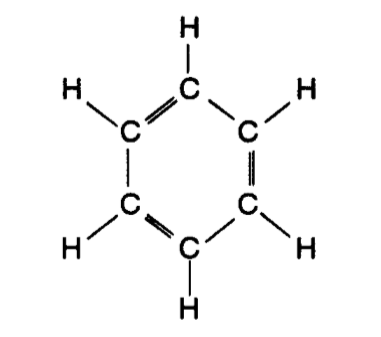
\includegraphics[width=0.5\columnwidth]{idrocarburi.png}
	\caption{ 	\label{idro}
		Struttura tipica degli idrocarburi aromatici.
	}
\end{figure}
Gli idrocarburi aromatici sono caratterizzati dalla presenza di almeno un anello benzenico. Hanno una struttura simile alla grafite (fig. \label{idro}), che è spesso considerata il genitore di tutti questi composti.
\begin{figure}[h!] 
	\centering
	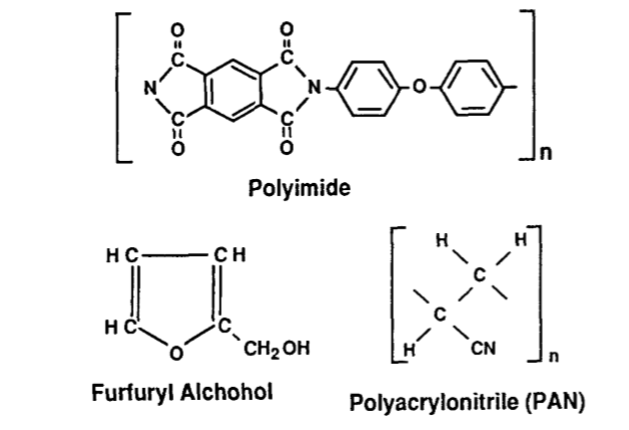
\includegraphics[width=0.8\columnwidth]{polymers.png}
	\caption{ 	\label{poly}
		 Nella figura abbiamo 3 importanti polimeri: il Poliimmide, l'Alcool furfurilico, il poliacrilonitrile.
	}
\end{figure}
I polimeri invece sono macromolecole organiche, che contengono in più, rispetto agli idrocarburi aromatici, altri elementi oltre al carbonio e l'idrogeno quali il cloro, l'ossigeno o l'azoto, il che li rende più pesanti (fig. \ref{poly}). Per eliminare gli atomi in più il processo di pirolisi risulta essere più complesso del primo.
La pirolisi è sostanzialmente un ciclo frigorifero. La molecola è riscaldata lentamente in un ambiente con gas inerte o riducente (che non ossida), fino ad una temperatura che può arrivare ai $1300 ^\circ C$. Il materiale organico viene scomposto in un residuo carbonioso ed i composti volatili prodotti nel processo si diffondono nell'atmosfera. Il processo è complesso e diverse reazioni possono avvenire contemporaneamente come la deidrogenazione, la condensazione e l'isomerizzazione. La pirolisi è di solito un processo lento. La sua durata può variare notevolmente, a seconda della composizione del prodotto finale, del tipo di molecola di partenza, dello spessore del materiale e di altri fattori.
\subsection{Highly oriented pyrolytic graphite}
Nei laboratori di ricerca sui materiali, il materiale grafitico di alta qualità più comunemente utilizzato oggi è la highly oriented pyrolytic graphite (HOPG), che viene preparata dalla pirolisi degli idrocarburi a temperature superiori a $2000 K$ e successivamente viene trattata a temperature più elevate. Quando lo stress viene ricotto al di sopra di $3300 K$ l'HOPG mostra proprietà elettroniche, di trasporto, termiche e meccaniche vicine a quelle della grafite monocristallina, dato che mostra un grado molto alto di allineamento dell'asse c. 
\subsection{Kish grafite}
La grafite "kish" è un tipo di grafite monocristallina sintetica comunemente usata nelle indagini scientifiche. I cristalli di grafite Kish si formano sulla superficie del ferro ad alto contenuto di carbonio in fase di fusione e vengono raccolti sottoforma di cristalli da tali soluzioni. Le scaglie di grafite kish sono spesso più grandi delle scaglie di grafite naturale, il che rende la grafite kish il materiale più scelto quando sono necessari grandi fiocchi monocristallini. I fiocchi monocristallini migliori attualmente disponibili hanno un diametro di circa 1 mm.
\subsection{Grafite whiskers}
I grafite whiskers sono formati attraverso una scarica posta ai capi di due elettrodi di carbonio usando $75-80 V e 70-76 A$. Il diametro dell'elettrodo positivo è inferiore a quello dell'elettrodo negativo e la scarica viene effettuata in un ambiente con gas inerte ad alta pressione ($92 atm$). Come risultato si formano tali grafite whiskers arrotolati, lunghi fino a $3 cm$. I whiskers che si formano hanno un'eccellente riproduzione del reticolo cristallino, un'elevata conducibilità elettrica e un alta elasticità: sin dalla loro scoperta, i grafite whiskers rappresentano il punto di riferimento rispetto al quale confrontare le prestazioni delle fibre di carbonio. 

\section{Reticolo cristallino}
\subsection{Struttura del reticolo}
\begin{figure}[h!] 
	\centering
	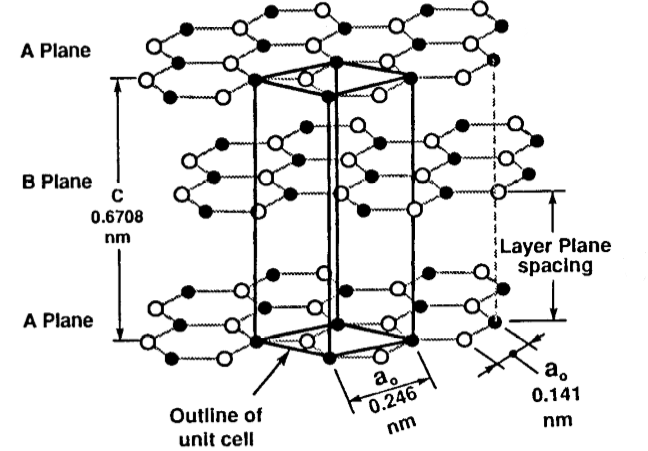
\includegraphics[width=0.8\columnwidth]{ABAB.png}
	\caption{ 	\label{AB}
		Struttura cristallina della grafite.
	}
\end{figure}
Il reticolo cristallino della grafite è composto di piani paralleli formati da atomi di carbonio arrangiati a formare una rete di esagoni, come si può notare in fig. \ref{AB}.
Nel caso della grafite il carbonio è in ibridizzazione di tipo $sp^2$, che genera tre legami $\sigma$ forti che giacciono in un piano, formando un triangolo, ed un legame debole $\pi$ perpendicolare al piano. Ogni atomo di carbonio che giace su uno strato è legato tramite legami covalenti ad altri tre, e tale struttura genera un foglio di grafite. I fogli di grafite sono tenuti insieme dalle forze di Van der Waals, che sono forze deboli, e ciò è la causa del fatto che i fogli si rompono facilmente fra di loro. 
I piani paralleli sono generalmente a due a due simili, creando una disposizione detta di tipo "ABAB". Facendo riferimento agli atomi in figura, in una cella unitaria (la struttura evidenziata formante un parallelepipedo a base quadrata) vi sono atomi che giacciono l'uno sopra all'altro sullo stesso asse, parallelo all'asse $c$.  Al contrario, i loro primi vicini non hanno un corrispettivo atomo sul piano consecutivo. La distanza tra un piano di tipo A ed un piano di tipo B è di $r_{AB}=\SI{3.3539}\angstrom$ ed i parametri di reticolo sono $a= \SI{2.462}\angstrom \: e \: c= \SI{6.708}\angstrom$. La distanza fra i due atomi di carbonio più vicini è di $r_{CC}=\SI{1.421}\angstrom$.
Il disordine tende ad avere dei piccoli effetti sul parametro di reticolo $a$, per lo più perchè il legame $C-C$ nel piano è molto forte e lo spazio fra i primi vicini è molto piccolo. Tuttavia, il disordine ha un effetto significativo perchè confrontabile con le dimensioni del reticolo e a causa del debole legame interplanare. Una conseguenza del piccolo valore di $r_{CC}$ è l'improbabilità che le impurità entrino in sostituzione dei siti del reticolo nel piano: è più probabile che occupino piuttosto una posizione interstiziale tra i piani del livello.

 \subsection{Reticolo romboedrico}
In casi meno frequenti, i piani vanno a comporre una struttura del tipo "ABCABC". Questa particolare struttura ha una cella unitaria di forma romboedrica (fig \ref{ABC}), da cui il nome grafite romboedrica. I parametri di reticolo sono $a= \SI{25.66}\angstrom$, $c = \SI{100.62}\angstrom$. 
Essa può essere considerata come un difetto di impilamento della grafite esagonale. La grafite romboedrica non può essere isolata in forma pura (sia la grafite naturale che quella sintetizzata contengono poco meno del $40\%$ di grafite romboedrica in combinazione con grafite esagonale). Viene prodotta da una deformazione tangenziale della grafite esagonale, dunque ha la proprietà di trasformarsi progressivamente nell'impilamento ABAB per riscaldamento oltre $T=1600 K$. Per questo è una tipologia di grafite rara: è termodinamicamente instabile. 
\begin{figure}[h!] 
	\centering
	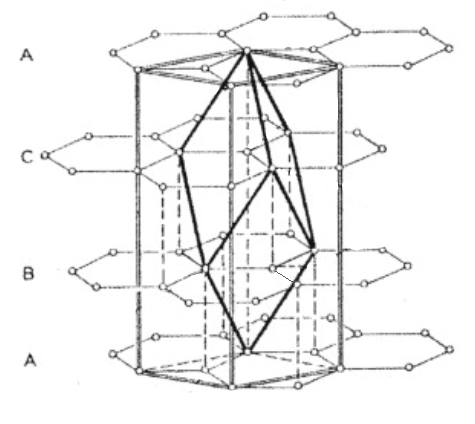
\includegraphics[width=0.6\columnwidth]{ABCABC.png}
	\caption{ 	\label{ABC}
		Struttura cristallina della grafite romboedrica.
	}
\end{figure}

\subsection{Dispersione fononica}
Per descrivere le relazioni di dispersione fononica della grafite, viene utilizzata la zona Brillouin 
\begin{figure}[h!] 
	\centering
	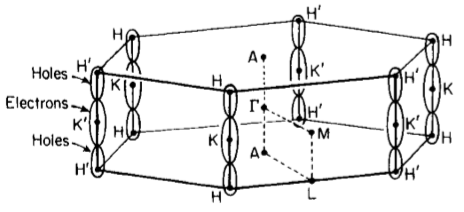
\includegraphics[width=0.6\columnwidth]{brillouingrafite.png}
	\caption{ 	\label{Br}
		Prima zona di Brillouin e dispersione elettronica.
	}
\end{figure}
mostrata in Fig. \ref{Br}. \\
Il punto $K$ in figura è la posizione del livello di Fermi per la grafite $2D$ ed il punto di degenerazione delle bande di conduzione e di valenza causato dalla simmetria del sistema. \\
Si  riportano di seguito i dati dello studio condotto sulla dispersione fononica da Maultzsch et al.\cite{Mault} usando lo scattering anelastico a raggi X.
Il calcolo teorico delle relazioni di dispersione è stato effettuato tramite l'approssimazione di gradiente generalizzato (GGA). Le frequenze calcolate nei punti K e M differiscono fino a $300 cm^{-1}$, determinando grandi differenze nelle relazioni di dispersione dei fononi calcolate sia nella loro forma generale che per le pendenze.
Per semplicità usiamo i termini LO e TO  per i rami ottici che sono strettamente longitudinali e trasversali, mentre il ramo acustico è detto LA.
La larghezza di banda del ramo TO è $320 cm^{- 1}$. I dati mostrano che i rami LO e TO si incrociano nel punto K e in M.
I punti in figura mostrano la dispersione fononica della grafite misurata sperimentalmente; nel punto M il ramo di dispersione fononica ottico e acustico longitudinale sono a frequenze pari a $1323 cm ^ {- 1}$ e $1290 cm ^ {- 1}$, rispettivamente. Quest'ultimo ramo è in ottimo accordo con le misurazioni. Nel punto K si è ottenuto per il ramo TO una frequenza di $1265 \pm 10 cm^{-1}$ da un'estrapolazione della misurazione effettuata, indicata dalla linea tratteggiata rossa in Fig. \ref{phonon}.

\begin{figure}[h!] 
	\centering
	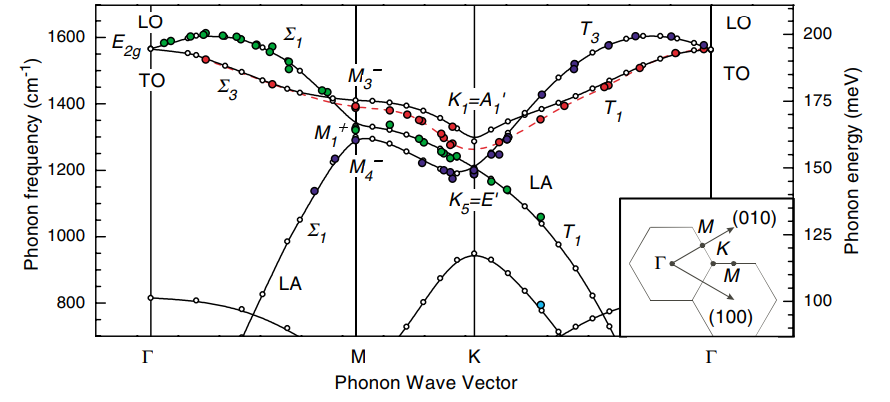
\includegraphics[width=1\columnwidth]{fononegrafite.png}
	\caption{ 	
		Curve di dispersione fononica della grafite. Ogni linea proviene dall'esecuzione di un fit polinomiale dei dati. I punti colorati sono i dati sperimentali per il ramo LO, TO e LA. I dati sperimentali del ramo TO sono collegati da un fit polinomiale cubico (linea tratteggiata). L'errore sperimentale è inferiore alla dimensione dei simboli. I punti vuoti sono le frequenze calcolate teoricamente dei fononi. Inserto: zona di Brillouin della grafite nel piano basale con i punti ad alta simmetria $\Gamma$, K e M. Le frecce indicano i vettori del reticolo reciproco.
	} \label{phonon}
\end{figure}




\section{Proprietà fisiche}
I materiali come la grafite pirolitica, il carbonio vetroso, ed altri simili, sono aggregati dei cristalli di grafite. Quest'ultimi possono variare molto in grandezza con differenti proprietà fisiche, infatti nel caso in cui gli aggregati siano composti da pochissimi cristalli di grafite (come ad esempio la fuliggine) le proprietà fisiche sono attribuite all'area superficiale.
Alcuni aggregati possono essere relativamente grandi, privi di difetti e con piani allineati tra loro, in tal caso la struttura e le sue proprietà corrispondono a quelle del cristallo di grafite ideale. Molto spesso la grafite pirolitica rispecchia il cristallo di grafite ideale. In altri aggregati invece, i cristalliti hanno un orientamento casuale, un esempio è la grafite turbostratica. In tali casi, il cristallo risulta essenzialmente isotropico. 
La particolare struttura cristallina della grafite la rende notevolmente anisotropica, cioè le proprietà del materiale possono variare considerevolmente se misurate lungo le direzioni \textbf{a} x \textbf{b} (all'interno di un piano) o nella direzione \textbf{c} (perpendicolare ai piani). 
La densità del cristallo perfetto è: $\rho=2,26 g / cm^3$ a $T = 300 K$ e $p = 1 atm$. Questa è la densità teorica, ma la maggior parte dei materiali composti di grafite avrà densità più basse a causa della presenza di imperfezioni strutturali come la porosità, i gap di atomi di carbonio nel reticolo e le dislocazioni; questa è una caratteristica vantaggiosa specialmente nelle applicazioni aerospaziali. La grafite può essere considerata la più refrattaria di tutti gli elementi, grazie al suo punto di fusione (o piuttosto di sublimazione) a $1 atm$ di $4000K$.
Il calore specifico molare della grafite è fra i $8.033 - 8.635 J/mol \cdot K$ a $25 ^\circ C$ e aumenta con la temperatura, con la seguente relazione (T in Kelvin)
\begin{equation}
C=4.03+(1.14 \cdot 10^{-3})T- \frac{(2.04 \cdot 10^5)}{T^2}
\end{equation}

Il calore specifico aumenta rapidamente con la temperatura fino a $1500 K$, dove si stabilzza a circa $2,2 \: kJ / kg \cdot K$ come mostrato in fig. \ref{cal}. \\
\begin{figure}[h!] 
	\centering
	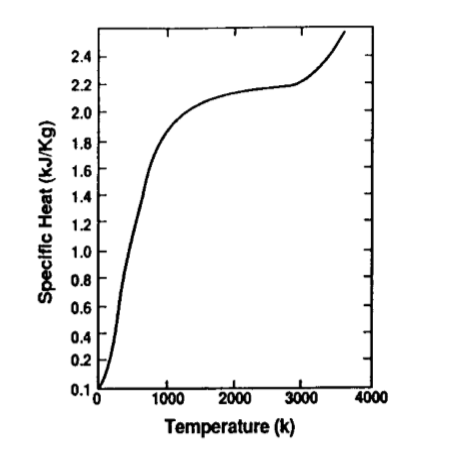
\includegraphics[width=0.6\columnwidth]{calspecgraf.png}
	\caption{ 	\label{cal}
		Andamento del calore specifico in funzione della temperatura.
	}
\end{figure}

Il valore medio della conducibilità termica per le direzioni \textbf{a} x \textbf{b} del reticolo cristallino della grafite pirolitica commerciale è $390 W/m \cdot K$ circa. Si tratta di un valore elevato e perciò la grafite può essere considerata un buon conduttore termico nelle direzioni \textbf{a} x \textbf{b}, paragonabile ai metalli ad alta conducibilità e alla ceramica. Nella direzione \textbf{c} è approssimativamente $2,0 W/m \cdot K$ e, in quella direzione, la grafite è un buon isolante termico, paragonabile alla plastica fenolica.
La grafite può essere considerata un semimetallo, cioè un conduttore nel piano basale e un isolante normale al piano basale: la sua struttura a bande è tale che la banda di valenza più alta si sovrappone alla banda di conduzione più bassa vuota di circa $36 meV$ ed i quattro elettroni spaiati delocalizzati formano una banda di conduzione parzialmente piena tra i piani basali dove, nel caso di presenza di un campo elettrico esterno, si possono muovere seguendo il pattern d'onda del campo. Di conseguenza, la resistività elettrica della grafite, lungo la direzione parallela ai piani basali (direzioni \textbf{a} x \textbf{b}), è bassa e il materiale è un conduttore relativamente buono di elettricità. 
Nella direzione \textbf{c}, la spaziatura tra i piani è relativamente grande, e non vi è possibilità per gli elettroni di muoversi da un piano all'altro, di conseguenza la resistività elettrica in quella direzione è alta e il materiale è considerato un isolante elettrico. 

\section{Applicazioni possibili}

A causa delle sue proprietà termiche e strutturali, la grafite è utilizzata in quasi tutti i settori commerciali e industriali. \\

La più grande applicazione di grafite modellata è la produzione di elettrodi per la lavorazione dell'acciaio e dell'alluminio. Gli elettrodi sono una delle primissime applicazioni e sono stati realizzati con lo stesso processo per quasi un secolo. \\
L'utilizzo maggiore di questi elettrodi è nella produzione di acciaio nei forni elettrici ad arco (fig. \ref{arc}), principalmente per la bonifica dei rottami ferrosi. \\
\begin{figure}[h!] 
	\centering
	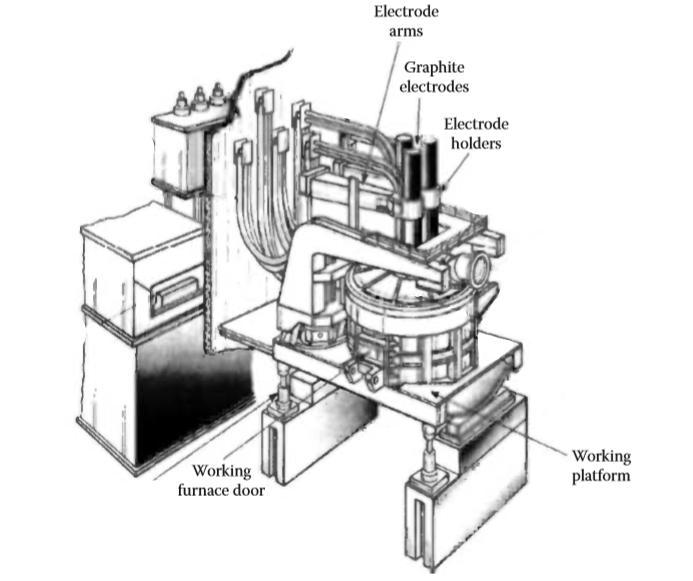
\includegraphics[width=0.6\columnwidth]{electricarc.png}
	\caption{ 	\label{arc}
		Rappresentazione grafica di un forno elettrico ad arco.
	}
\end{figure} 
La grafite modellata ha numerose applicazioni nella lavorazione di metalli ferrosi e non ferrosi e leghe come rame, rame-nichel, ottone, bronzo, zinco, leghe di alluminio, nichel e sue leghe, metalli preziosi e ferri duttili.\\
 Nel 1947, Bardeen, Brattain e Shockley dei laboratori Bell Telephone dimostrarono l'utilità dei transistor di germanio. Quell'anno segnò l'inizio dell'industria dei semiconduttori a stato solido.\\

Le applicazioni elettriche della grafite modellata sono dovute alla buona conducibilità elettrica e la capacità di resistere al calore con il minimo danno. Fra le maggiori applicazioni attuali ritroviamo la grafite negli elettrodi per illuminazione, elettroerosione (EDM) e forni elettrici ad arco, nelle componenti delle celle a combustibile, in anodi, catodi ed altre batterie avanzate.\\

Nelle applicazioni meccaniche si sfrutta la grafite modellata a grana fine, ad alta densità e a bassa porosità. Essa è ampiamente utilizzata per cuscinetti e tenute, in particolare nelle applicazioni ad alta temperatura (fino a $600 ^\circ C$) dove i lubrificanti liquidi convenzionali si degradano rapidamente. Ha eccellenti proprietà lubrificanti e di attrito, è chimicamente resistente, la sua alta conducibilità termica aiuta a dissipare il calore generato dall'azione dello sfregamento e, a temperature elevate ($> 500 ^\circ C$)), la sua resistenza alla compressione è superiore a quella della maggior parte degli altri materiali ingegneristici. \\

Un gruppo specializzato di applicazioni riguarda i sistemi aerospaziali che includono ugelli per razzi, dove le prestazioni della grafite modellata si sono rivelate eccellenti, grazie alla sua resistenza ad alte temperature, all'erosione e agli shock termici .\\

Per ciò che concerne le applicazioni chimiche, la grafite modellata ha utilizzi in aree in cui la resistenza agli agenti chimici è il fattore principale. Tali applicazioni si trovano nei reattori, apparecchiature per la sedimentazione di vapori chimici e anodi per condotte, piattaforme petrolifere, linee di alimentazione DC, costruzioni stradali e di edifici.\\

Per quanto riguarda le applicazioni nucleari, la grafite modellata è uno dei materiali migliori nel campo della fissione nucleare poiché combina un'elevata efficienza di schermazione dei neutroni e una bassa sezione di assorbimento degli stessi, una buona resistenza meccanica e chimica, malleabilità e costi relativamente bassi. Tuttavia, la radiazione nucleare colpisce il reticolo cristallino che si distorce a causa delle collisioni con i neutroni ed altre particelle energetiche. Di conseguenza, le proprietà risultano modificate. La forza e la durezza generalmente aumentano e le variazioni nelle distanze interatomiche diventano particolarmente evidenti ad alte temperature. \\
La grafite modellata viene anche utilizzata nei reattori di fusione come rivestimenti interni, il suo basso numero atomico è un fattore importante nel ridurre l'interferenza con la reazione di fusione. 

\chapter{Grafene}
Il grafene è essenzialmente un singolo strato di grafite sotto forma di un reticolo di atomi di carbonio disposti a nido d'ape legati fra loro grazie alla configurazione $sp^2$. Tutti i legami interatomici sono pari a $\SI{1,42}{\angstrom}$. 
Costituisce inoltre la struttura base dei nanotubi di carbonio. Lo scopo dei fisici quando fu scoperto era quello di studiare una quasiasi manifestazione fisica della meccanica quantistica in due dimensioni, dunque non ebbero altra scelta che fabbricare sistemi a due dimensioni confinando artificialmente strutture 3D in un piano. In questo modo lo spettro dell'energia è confinato ed effettivamente risulta ridotto a un singolo livello. La sintesi del grafene generò un cristallo stabile a temperatura ambiente, con proprietà uniche nel suo genere. Per questo la sua scoperta suscitò ben più clamore dei nanotubi di carbonio.

\section{Sintetizzazione e scoperta}
Il grafene è stato isolato per la prima volta nel 2004 dai fisici Geim e Novoselov sintetizzandolo mediante il metodo Scotch-Tape. Nel 2010 il premio Nobel per la fisica è stato assegnato ad entrambi, per la loro pioneristica ricerca sulla struttura e le proprietà del grafene. L'idea di ottenere il grafene separandolo dalla grafite è ben più antica, infatti risale agli inizi del XX secolo.
\begin{figure}[h!] 
	\centering
	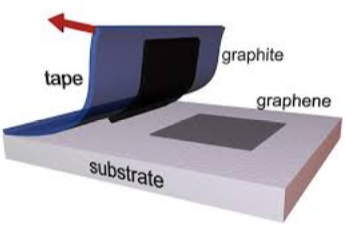
\includegraphics[width=0.6\columnwidth]{scotchtape.png}
	\caption{ 	\label{tape}
		Semplificazione della metolodogia di sitetizzazione Scotch-tape.
	}
\end{figure}
L'azione di sintetizzazione della grafite utilizzando la tecnica di esfoliazione meccanica resa popolare dai premi nobel, consiste essenzialmente nel rimuovere pochi strati di grafite dai cristalli usando nastro adesivo, trasferendolo su un substrato di $SiO_2$ stabile. Tale tecnica è stata il primo passo che ha portato all'isolamento sperimentale e al rilevamento di un monostrato di grafite nel 2004 \ref{tape}. Questo esperimento ha avviato un'ondata di interesse senza precedenti nella comunità della fisica della materia e oltre. \\

Negli ultimi anni, i ricercatori hanno compiuto notevoli passi avanti per sviluppare metodi di produzione per il grafene. Attualmente sono disponibili nuovi diversi metodi di sintesi:
\begin{itemize}
	\item Tecnica CVD (chermical vapor deposition): che verrà approfondita nel capitolo riguardante i nanotubi di carbonio; 
	\item Crescita epitassiale: La decomposizione termica del $SiC$ consiste nel riscaldare il campione in ultra-alto vuoto (UHV) a temperature comprese tra 1273 e 1773 K, che fanno sì che il $Si$ si sublimi lasciando una superficie ricca di carbonio. Questa tecnica è in grado di generare strati sottili di grafene.
	\item Riduzione chimica dell'ossido di grafite ($GO$): La riduzione di una sospensione colloidale di fogli di ossido di grafite in acqua con idrazina idrato, determina la loro disgregazione e la successiva formazione di fogli sottili di grafene con una grande area superficiale.
	\item Sintesi solvotermica: i sottili fogli di grafene compatto sono stati isolati dalla grafite sfusa mediante scissione micromeccanica.
	\item Esfoliazione termica: l'esfoliazione viene spesso ottenuta introducendo ulteriori forze esterne per superare la forza di van der Waals tra gli strati di grafite. Durante la processazione termica dell'ossido di grafite o di atri composti, la pressione dovuta alla decomposizione dei gruppi funzionali tra gli strati della grafite supera le attrazioni di van der Waals e si traduce in esfoliazione.
\end{itemize}

\section{Reticolo cristallino}

\subsection{Struttura del reticolo}
\begin{figure}[h!] 
	\centering
	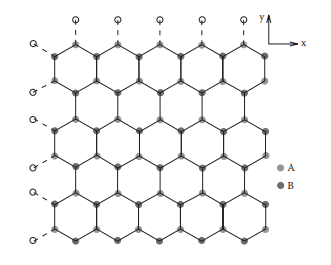
\includegraphics[width=0.6\columnwidth]{praghene.png}
	\caption{ 	\label{pra}
		Struttura del grafene.
	}
\end{figure}
Il grafene è costituito da atomi di carbonio disposti in un reticolo a nido d'ape, come illustrato nella fig. \ref{pra}. Ogni atomo di carbonio possiede quattro elettroni di valenza, tre dei quali interagiscono chimicamente con i primi vicini e formano forti legami $\sigma$ nel piano, con conseguente ibridazione $sp^2$ degli orbitali atomici. L'elettrone libero rimanente forma un legame $\pi$ debole, diretto perpendicolarmente al piano, creando un orbitale $p_z$. L'eletrone può saltare da un atomo all'altro e generare la propagazione di una corrente di carica attraverso il cristallo. Un modello che descrive questo fenomeno prevede che gli elettroni di conduzione saltino (con salto di ampiezza  $\gamma_0 \approx 3 eV$)  solo tra primi vicini (separati da una distanza di $\approx 0.1 nm$), e tale modello risulta sufficiente per spiegare la maggior parte delle proprietà elettroniche del grafene.\\
La cella unitaria primitiva del reticolo esagonale (da cui può essere generato l'intero piano del grafene) è composta da due atomi \ref{label}.
\begin{figure}[h!] 
	\centering
	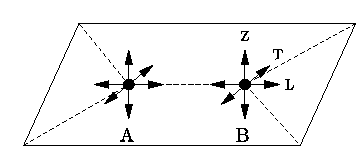
\includegraphics[width=0.6\columnwidth]{cellunit.png}
	\caption{ 	\label{label}
		Cella unitaria contenente due atomi appartenenti ai due sottoreticoli A e B; il moto degli atomi di carbonio nel grafene può essere lungo la direzione fuori dal piano (direz. Z),e le direzioni nel piano: trasversale (direz. T) e longitudinale (direz. L). 
	}
\end{figure}
Ciò implica l'esistenza di due corrispondenti sottoreticoli e un grado di libertà associato all'elettrone libero; il che può essere sia nel sottoreticolo A che nel sottoreticolo B. Questo grado di libertà agisce come uno pseudo-spin dell'elettrone: il sistema risulta descritto da una funzione d'onda a due componenti, che sono l'analogo degli spinori in teoria dei campi. Questa struttura garantisce agli elettroni un grado di libertà interno strettamente connesso con la fase di Berry (è la fase acquistata da uno stato quantistico a seguito di una variazione adiabatica ciclica dell'Hamiltoniana descrivente la dinamica del sistema). 

\subsection{Dispersione fononica nel grafene}
Poiché ci sono due atomi di carbonio, A e B, nella cella unitaria del grafene, si devono considerare 6 coordinate. L'equazione secolare da risolvere è quindi una matrice di rango 6, perciò si hanno 6 rami per la dispersione fononica. La relazione di dispersione dei fononi  nel grafene comprende tre rami acustici (A) e tre rami ottici (O). I modi sono associati ai moti degli atomi fuori dal piano (Z), longitudinale nel piano (L) e trasversale nel piano (T) \ref{label}.\\
\begin{figure}[h!] 
	\centering
	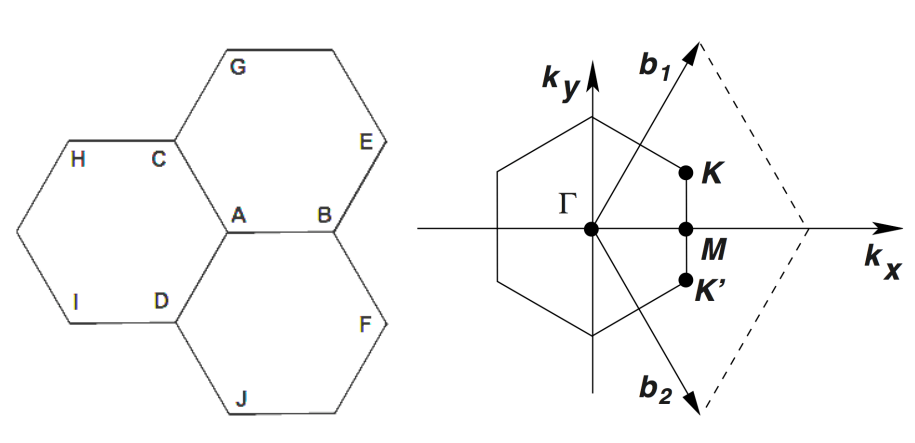
\includegraphics[width=0.6\columnwidth]{primitivecellgraph.png}
	\caption{ 	\label{labe}
		\textit{(sinistra)} - Struttura cristallina del grafene nel reticolo diretto; \textit{(destra)} - prima zona di Brillouin del grafene ed i suoi punti di simmetria.
	}
\end{figure}
La figura \ref{fog} mostra i rami di dispersione fononica del grafene. I tre rami che scaturiscono dal punto Gamma della zona di Brillouin\ref{labe}, corrispondono ai modi acustici calcolati, sempre prendendo in esame le relazioni di dispersione trovate utilizzando le codizioni di Born-von Karman. Essi corrispondono al modo uscente dal piano (ZA), il modo trasversale nel piano (TA) e longitudinale nel piano (LA), elencati in ordine crescente di energia. I restanti tre rami corrispondono ai modi ottici: il modo fuori piano (ZO) e i due modi nel piano (TO) e (LO). Mentre i modi TA e LA mostrano una dispersione lineare attorno al punto $\Gamma$ per piccoli spostamenti, il modo ZA mostra una dispersione di energia $q^2$ che è spiegata in Saito et al.\cite{Saito} come conseguenza della simmetria $D_{6h}$, ossia la simmetria di tipo esagonale, riscontrata nel grafene. Un'altra conseguenza di tale simmetria sono le degenerazioni nei punti M e K delle linee nei modi ZA / ZO e LA / LO.
 \begin{figure}[h!] 
 	\centering
 	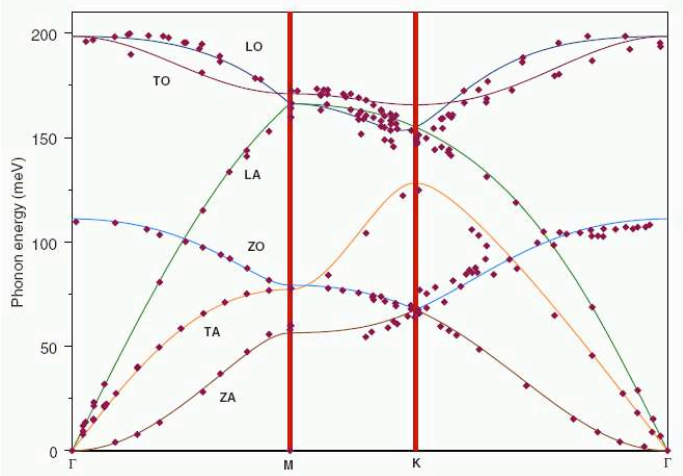
\includegraphics[width=0.8\columnwidth]{phografe.png}
 	\caption{ 	\label{fog}
 		Struttura cristallina esagonale di una cella primitiva del grafene e i suoi primi vicini; (destra) prima zona di Brillouin del grafene ed i suoi punti di simmetria.
 	}
 \end{figure}
Sono stati riportati in figura inoltre i dati dell'esperimento effettuato da Gray et al.\cite{Gray}, utilizzarono la tecnica di scattering anelastico a raggi X, e risultano molto in accordo con le previsioni teoriche.
Le maggiori discrepanze tra i dati sperimentali ed il modello Born sono per le modalità TO e LO, a causa del trascurare le interazioni elettrone-fonone.

\section{Proprietà fisiche e utilizzi}
A causa delle sue proprietà chimiche e fisiche uniche, il grafene trova applicazioni per componenti elettronici inclusi circuiti integrati, optoelettronica, sensori ad effetto Hall, assorbimento / modulazione ottica, rilevamento di luce infrarossa, celle fotovoltaiche, elettrodi, celle a combustibile, supercondensatori, sensori di assorbimento molecolare e dispositivi piezoelettrici.\\

Il grafene mostra eccezionali caratteristiche di trasporto, incluso un effetto di sintonizzazione su un campo elettrico esterno presente, cioè la capacità di regolare continuamente la densità dei propri portatori di carica, alternando in modo diverso elettroni e lacune, tramite l'applicazione di una tensione dovuta ad un campo esterno. Sono stati anche misurati dei moti di carica $\mu$ molto elevati, probabilmente dovuti al fatto che su grandi distanze i portatori di carica attraversano il materiale senza essere scatterati: $\mu$ supera i $10^4 \frac{cm^2}{V \cdot s}$ per il grafene depositato su un substrato di $SiO_2$ e i $10^5 \frac{cm^2}{V \cdot s}$ per il grafene in sospensione, il più alto valore mai riportato per un semiconduttore a temperatura ambiente. \\
Il grafene è degno di nota, per le sue proprietà di tipo ottico, meccanico e termico. È otticamente quasi trasparente nell'intero spettro della luce visibile, che assieme alla natura chimica del carbonio rende il grafene un candidato ideale per agire come supporto su cui manipolare molecole biologiche come il DNA. È allo stesso tempo eccezionalmente forte (più di 100 volte più forte dell'acciaio con un carico di rottura dell'ordine di $40 N / m$) e molto flessibile. La sua conducibilità termica è impressionante (dell'ordine di $1000 \: \frac{W}{m \cdot K}$), superando anche quella del rame a temperatura ambiente, il che consente agli elettrodi di grafene di diventare efficienti dispositivi di rimozione del calore, per rimuovere le quantità sempre maggiori di calore dissipate dai moderni dispositivi elettronici. Il grafene è anche impermeabile alle molecole di gas più piccole, come l'elio, aprendo la strada alle applicazioni dei sensori di gas.\\
A causa della sua elevata resistenza, della buona conducibilità e dell'elevata stabilità termica, il grafene viene utilizzato come riempitivo in composti polimerici e come modello per la sintesi di nanoparticelle metalliche, che hanno applicazioni in sensori elettrochimici. Inoltre, i nanomateriali semiconduttori di grafene hanno un largo impiego in dispositivi come batterie agli ioni di litio, celle solari e supercondensatori. Il grafene, in particolare sotto forma di nanostrip e nanomesh, è utilizzato in vari componenti elettronici come transistor ad effetto di campo, circuiti integrati e dispositivi di memoria. Grazie alla sua struttura planare 2D, il grafene costituisce un'ottima piattaforma per la rilevazione di molecole chimiche e biologiche, in quanto l'azione di assorbimento di poche molecole può portare a un cambiamento misurabile della resistenza.\\
L'elettronica dei semiconduttori è generalmente divisa in due principali campi di applicazione: dispositivi logici digitali, che sono dominati dalla tecnologia Si-MOSFET, e dispositivi a radiofrequenza, che sono diventati sempre più rilevanti con l'avvento delle comunicazioni wireless.
Le sue prospettive in quest'ultimo sono molto incoraggianti: le prestazioni in radiofrequenza  riguardano l'amplificazione di segnali. La frequenza limite è il suo motivo principale di merito, infatti i transistor di grafene dimostrano di raggiungere frequenze di taglio di 100 GHz.\\
Il grafene gioca un ruolo incredibilmente importante nella realizzazione dei transistor \ref{trans}. \\
 \begin{figure}[h!] 
	\centering
	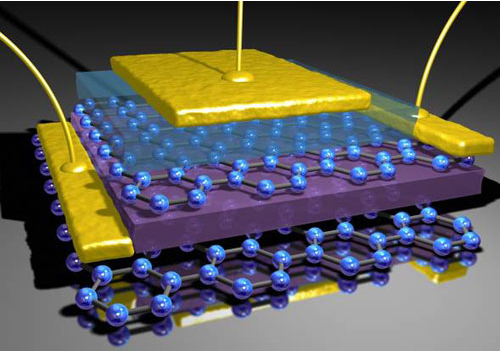
\includegraphics[width=0.5\columnwidth]{transistor.png}
	\caption{ 	\label{trans}
		Transistor a effetto di campo fatto da grafene. In figura notiamo tre placche gialle, che sono il Source, il Top Gate ed il Drain, in ordine di apparizione da sinistra verso destra. Gli strati viola sono strati isolanti di $SiO_2$
	}
\end{figure}
La cosiddetta legge di Moore, attesta che la potenza di calcolo dei processori raddoppia ogni 18 mesi. La dimensione dei transistor di silicio stava raggiungendo il limite inferiore critico in cui gli effetti quantistici si prevede che distruggano la fenomenologia dei trasporti classica, che regola il comportamento dei transistor convenzionali ad effetto di campo.\\
Si è quindi creata la necessità di un altro materiale in grado di superare questi limiti e il grafene si è rivelato un candidato serio per questo compito. Il suo vantaggio più significativo rispetto al silicio è che può essere rimpicciolito a dimensioni inferiori di esso di un ordine di grandezza (2-3 nm). Altri vantaggi includono una resistenza $V_{top}/I_{on}$ del transistor molto più bassa rispetto ai Si-MOSFET e una velocità di saturazione molto più elevata a causa delle frequenze più alte richieste nel grafene. Naturalmente, l'alta mobilità elettrica già dichiarata del grafene è anche un buon punto a favore poiché aumenta la velocità di switching.

\chapter {Diamante}
Per iniziare la trattazione delle forme allotropiche del carbonio con ibridazione $sp^3$ si analizza il diamante.
Esso è un allotropo meta-stabile del carbonio con gli atomi disposti in struttura cristallina fcc (face-centered cube). I diamanti si formano a una pressione di 5-6 GPa, a temperature che variano tra 900-1400 K. Il diamante è meno stabile della grafite a temperatura ambiente, per questo la conversione del diamante in grafite in condizioni standard è molto semplice da ottenere. 
\section{Sintetizzazione e scoperta}
\subsection{Scoperta}
Il diamante è conosciuto dall'uomo sin dai tempi preistorici ed è stato apprezzato da sempre per essere una gemma di eccezionale bellezza, brillantezza e lucentezza. La parola diamante deriva il suo nome dall'alterazione della parola latina \textit{adamas} che significa "indomabile" o "invincibile", riferendosi alla sua durezza. Per oltre 2000 anni, i diamanti sono stati ricavati dalla ghiaia dei fiumi sottoforma di cristalli.
Il diagramma di fase del carbonio \ref{fig:dyagramphase} mostra che il diamante si forma a temperature e pressioni molto elevate. Ciò significa che il diamante si cristallizza in natura a grandi profondità, grazie ai processi geologici, sotto la superficie terrestre. Queste condizioni esistono generalmente a più di 150 chilometri sotto la crosta terrestre, ossia nel mantello. Il materiale sedimentato organico entra in tale regione, dove il carbonio in condizioni estreme si cristallizza in diamante. I diamanti vengono trasportati sulla superficie terrestre da frammenti di mantello e magma fuso, che affiorano durante le eruzioni vulcaniche attraverso dei tubi conici chiamati “camini kimberlitici”. Il diamante naturale si trova principalmente nei camini di kimberlite delle zone vulcaniche ormai spente dove viene generalmente estratto.
\subsection{sintetizzazione}
Il diamante sintetico si crea principalmente allo stesso modo dei diamanti naturali. La grafite viene riscaldata a temperature superiori a $1500^\circ C$ e a circa 60.0000 atm di pressione in un apparato apposito. L'aggiunta di piccole quantità di catalizzatori metallici, come ferro o nichel, accelera la reazione e riduce la pressione e la temperatura richieste. Nella formazione dei diamanti, delle impurità si possono intrappolare nel reticolo cristallino che si forma. Questo è il motivo per cui i diamanti possono essere colorati.
\subsection{Dalla grafite esagonale al diamante cubico}
I risultati degli esperimenti condotti da Xie et al. \cite{XIE} rivelano un nuovo meccanismo cosiddetto di "ondulamento e slittamento simile ad un onda", che governa la trasformazione dalla grafite esagonale al diamante cubico. Sulla base di questo meccanismo si dimostra che la distanza iniziale tra gli strati della grafite esagonale gioca un ruolo chiave per determinare la dimensione dei grani del diamante cubico. 
Impostiamo la pressione lungo la direzione \textbf{x} [2 1 0]. Il processo di trasformazione strutturale con distanza fra gli strati di 0,214 nm è mostrato in Fig. \ref{diamon}.\\
 \begin{figure}[h!] 
	\centering
	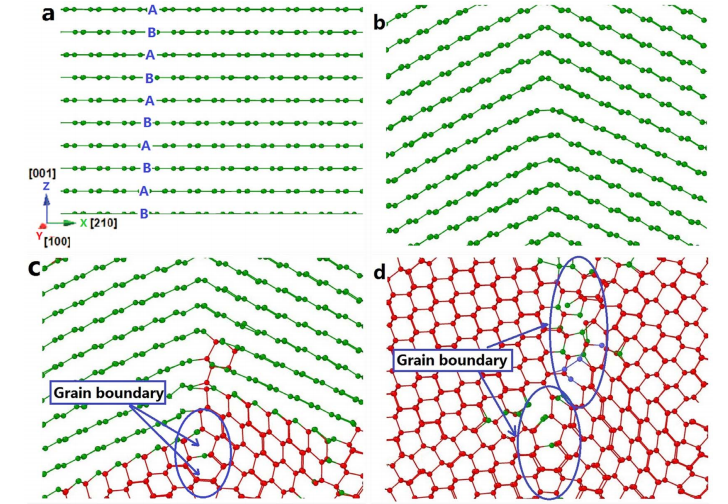
\includegraphics[width=0.8\columnwidth]{graphtodiamond.png}
	\caption{ 	\label{diamon}
		Trasformazione della grafite esagonale con distanza fra gli strati di 0,214 nm in diamante cubico policristallino. (a) Le sfere verdi e rosse rappresentano gli atomi che hanno rispettivamente tre e quattro primi vicini. (B) Sovrapposizione degli strati di grafite che si trasformano da "ABAB" a "ABCA" (grafite romboedrica); (C). Parti di grafite convertite in diamante cubico. (D). La grafite si trasforma completamente in diamante cubico policristallino. 
	}
\end{figure}
Gli strati di grafite si piegano in risposta ad una sollecitazione critica di compressione, e nel frattempo lo slittamento degli strati di grafite si sovrappongono trasformandosi da "ABAB" a "AAAA". Con l'aumentare della sollecitazione di compressione, l'angolo di inclinazione degli strati di grafite diventa sempre più grande; quando l'angolo di inclinazione raggiunge un determinato valore di $23,5^\circ$, l'ordine di impilamento degli strati di grafite si trasforma da "AAAA" a "ABCA". Quindi, la grafite romboedrica inizia a trasformarsi in diamante; gli atomi vicino al punto di instabilità formano un cosiddetto "bordo di grano" (\ref{diamon}-$(c)$). Di conseguenza, la grafite si trasforma in diamante (\ref{diamon}-$(d)$) con angolo di deformazione inferiore a $30^\circ$.
\subsection{Nucleazione da grafite romboedrica a diamante} \label{fif}
Un'altra metodologia per ricavare il diamante è attraverso il processo di nucleazione (un tipo di transizione di fase) da grafite a diamante. 
La compressione  della grafite romboedrica a temperature più elevate forma il diamante cubico (CD). Sebbene la pressione di transizione sia differente in base alla natura dei campioni di grafite, non si osserva nessuna formazione del diamante sotto ~12 Gpa. I nuclei di CD si formano in seguito allo spostamento degli atomi nel reticolo di grafite nel modo mostrato in fig. \ref{diamond}.\\
 \begin{figure}[h!] 
	\centering
	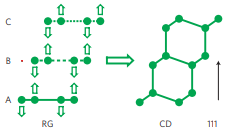
\includegraphics[width=0.6\columnwidth]{formdiamante.png}
	\caption{ 	\label{diamond}
		Stadio successivo: transizione da grafite con piani di tipo "ABCABC" al diamante.
	}
\end{figure}
L'instabilità dei piani basali nella conformazione del reticolo RG porta al CD. Tali distorsioni di piani di grafite sono state osservate in precedenti simulazioni e soddisfano le relazioni di orientamento tra cristalli di grafite e diamanti scoperti sperimentalmente \cite{Rustam}.
\section{Reticolo Cristallino}
\subsection{Struttura del reticolo}
Nel diamante, ogni atomo di carbonio è legato covalentemente a quattro altri atomi di carbonio da forti legami derivanti dall'ibridazione $sp^3$, i quali sono tutti e quattro di tipo $\sigma$ con angolo fra due legami di $109,5^\circ$ ed è disposto in modo tale da formare un tetraedro.
La struttura ideale del diamante è mostrata in Fig.\ref{mond}.\\
 \begin{figure}[h!] 
	\centering
	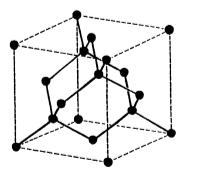
\includegraphics[width=0.6\columnwidth]{diaman.png}
	\caption{ 	\label{mond}
		Struttura del reticolo cristallino del diamante.
	}
\end{figure}
Ogni atomo di carbonio è circondato da altri quattro atomi di carbonio posti agli angoli di un tetraedro regolare, con parametro reticolare di $a_0 = \SI{3.567}{\angstrom}$. La struttura del diamante è quindi cubica e può essere vista come due strutture compenetranti di fcc spostate di (1/4, 1/4, 1/4)$\cdot a_0$ lungo la diagonale del corpo. A causa del forte legame $\sigma$ si avrà una distanza interatomica  breve ($r_{C-C} =\SI{1,45}{\angstrom}$), quasi il $10\%$ più grande rispetto alla grafite, tuttavia la densità atomica del diamante ($1,77\cdot 23 cm^{-3}$) è del $56\%$ superiore rispetto alla grafite, a causa dell'elevata anisotropia della struttura della grafite. 
Il cristallo di diamante è altamente simmetrico, il che lo rende pressochè isotropico.

\subsection{Dispersione fononica}
La legge sulla dispersione dei rami acustici e ottici nei cristalli di diamante per diverse polarizzazioni fononiche è stata studiata in precedenza mediante la spettroscopia a scattering anelastico di neutroni lenti e scattering anelastico a raggi X da Gorelik e Vasil'ev \cite{dimondi}. La figura \ref{phod} presenta dati sperimentali ottenuti da queste tecniche per la polarizzazione trasversale delle onde corrispondenti. Le linee continue rappresentano i nostri calcoli in un modello idealizzato entro l'approssimazione sinusoidale \ref{1} e \ref{2},
\begin{equation} \label{1}
\omega^2(k)=\omega_0^2-4 \frac{S^2}{a^2}sin^2(\frac{ka}{2}),  \: \: \: con \: S=a\sqrt{\frac{\left|\gamma\right|}{m}}
\end{equation}
\begin{equation}\label{2}
\omega^2(k)=2 \frac{S}{a}\left|sin(\frac{ka}{2})\right| ; 
\end{equation}
 con i seguenti parametri: \\
$S[100] = 12820 m/s,\\ S[111]=12060 m/s,\\ S[110]=12820 m/s,\\ \omega_0=\omega(\Gamma) =2,50 \cdot 10^{14} rad/s,\\ \: a=\SI{3,567}{\angstrom}$.

 \begin{figure}[h!] 
	\centering
	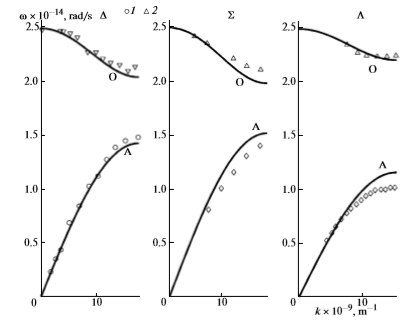
\includegraphics[width=0.7\columnwidth]{phodiamond.png}
	\caption{ 	\label{phod}
		Dispersione fononica nel diamante, in tre direzioni della prima zona di Brillouin differenti. Confronto di leggi di dispersione determinate in modo sperimentale (scattering di neutroni lenti e scattering a raggi X) del diamante. Dati sperimentali: (1) fononi acustici - pallini, (2) fononi ottici - triangoli. Le linee continue rappresentano le leggi d'approssimazione sinusoidale.
	}
\end{figure}

Come si vede in Fig.\ref{phod}, i dati sperimentali sono in accordo soddisfacente con la teoria se il parametro S, che sta per la velocità del suono nel diamante, è lo stesso per i due rami.

\section{Proprietà fisiche e applicazioni possibili}
\subsection{Proprietà}
Il diamante presenta una durezza molto elevata ed è molto denso ($3,5 g / cm^3$). Nel caso di un legame di tipo $sp^3$ non si presenta il fenomeno della delocalizzazione degli elettroni e questo rende il diamante un isolante. Il gap energetico del diamante infatti è $E_{gap} = 5.5 eV$, il che lo rende trasparente nella regione spettrale IR, visibile e UV.\\
È il materiale più duro conosciuto, il meno comprimibile e uno dei materiali più rigidi. È il miglior conduttore termico con un'espansione termica estremamente bassa e anche chimicamente inerte per la maggior parte degli acidi e alcali.\\
Le impurità nel diamante sono molto importanti a causa della variazione nelle proprietà elettriche e termiche; queste variazioni trovano applicazioni principalmente nei processi industriali. I migliori diamanti naturali contengono impurità con concentrazioni di circa una parte su $10^5$. Solo alcune specie chimiche (ad esempio, B, N) si possono inserire nel reticolo cristallino del diamante, e la concentrazione di tali impurità sostitutive sono molto basse (meno di una parte su $10^4$).\\
I diamanti sono stati storicamente classificati in base alle loro proprietà di assorbimento ottico, che sono determinate dalle impurità. I cosiddetti diamanti di tipo $1a$ mostrano un forte assorbimento nell'infrarosso. Ciò è causato da quantità piuttosto consistenti (fino allo $0,1\%$) di impurità, distribuite nel cristallo in modo disomogeneo, per lo più concentrate principalmente in piccoli agglomerati. La maggior parte dei diamanti naturali appartiene a questo gruppo.\\
I diamanti di tipo $1b$ contengono azoto come impurità sostitutive. Sebbene si formino raramente in natura, la maggior parte dei diamanti sintetici appartiene a questo gruppo.\\
I diamanti con la massima purezza sono di tipo $2a$, e presentano le proprietà intrinseche di semiconduzione con un gap di $5,47 eV$. I migliori diamanti sintetici sono di questo tipo e contengono meno impurità (in valore N) rispetto ai diamanti naturali.\\
I diamanti di tipo $2b$ sono drogati con il boro.\\
\subsection{Utilizzi}
Oltre agli usi tradizionali del diamante come gemme preziose, possiamo riassumere gli usi industriali che dominano i tempi attuali. Il diamante viene utilizzato negli utensili da taglio per ridurre l'usura, è un materiale ideale per strumenti di perforazione, di taglio e molatura. Essendo uno dei materiali più duri e abrasivi che si conoscano, il diamante può essere usato per lucidare e tagliare qualsiasi materiale, compresi altri diamanti. Alcuni esempi di applicazioni in ambito industriale sono la fabbricazione di punte da trapano, seghe con inserti in diamante e polvere abrasiva nelle smerigliatrici. Viene usato anche per il taglio e la lucidatura di pietre, vetro, marmo e granito. \\
In campo tecnologico questi cristalli sono usati nelle presse in diamante ed in molti strumenti ottici o di elettronica; l'estrema durezza unita alla trasparenza permette l'osservazione e lo studio delle alterazioni della materia, sottoposta a pressioni vicine a 2 milioni di atmosfere. In casi particolari, la superficie delle lenti ottiche viene protetta dall'abrasione con un sottilissimo film di diamante, applicato per mezzo di deposizione chimica. \\
Grazie alla sua elevatissima conducibilità termica, ben superiore a quella dell'argento o del rame, nella fabbricazione di semiconduttori di elevata potenza si usano talvolta sottilissimi strati di diamante come "basamento" del semiconduttore, rendendolo in grado di trasferire agevolmente il calore al contenitore. Esiste anche una pasta termoconduttiva a base di diamanti sintetici.

\chapter{Lonsdaleite}
La lonsdaleite è la versione del diamante di forma esagonale, invece che cubico come lo si conosce. Venne chiamato così in onore di Kathleen Lonsdale. Fu trovata per la prima volta in meteoriti contenenti grafite che colpirono la terra: fu identificata per la prima volta nel 1967 in un meteorite chiamato Meterorite del Canyon Diablo. A differenza del diamante, i legami intermedi sono in una conformazione "eclissata" (conformazione per la quale troviamo che gli atomi di carbonio ai vertici di un tetraedro ricoprono quelli appartenenti ad un altro tetraedro, lungo la direzione del legame fra gli atomi di carbonio centrale). La Lonsdaleite è del $58\%$ più dura del diamante per quanto concerne la direzione planare [1 0 0], e ha una resistenza alla pressione di indentazione di circa 152 GPa, che è molto più alta della resistenza del diamante di 97 GPa. 
\section{Sintetizzazione e scoperta}
La lonsdaleite fu scoperta per la prima volta nel meteorite Canyon Diablo, e furono dapprima identificate come delle piccole particelle molto dure (1891), e solo molto più tardi (1967) si scoprì invece che tali particelle contenevano grafite, diamante e lonsdaleite. 
La sua formazione all'interno del meteorite è stata attribuita al processo di trasformazione indotto da una copressione shock della grafite al momento dell'impatto con la terra. Da allora è stata segnalata in diverse meteoriti e nei sedimenti terrestri limitrofi e la loro formazione è sempre stata attribuita ad impatti di asteroidi, sia extraterrestri che sulla Terra. \\

La lonsdaleite è una dei primi allotropi del carbonio che fu sintetizzata in laboratoio in condizioni di pressione superiore a 13 GPa e di temperatura superiore a 1273 K.
Attualmente, può essere sintetizzata in campioni misti, in un ambiente di laboratorio a condizioni di pressioni e temperature alte (HPHT). Di solito la grafite è usata come materiale di partenza in tali esperimenti di sintetizzazione. 
La metodologia per ricavare la lonsdaleite maggiormente utilizzata è attraverso il processo di transizione di fase mediante nucleazione della grafite di tipo "ABAB".
La compressione statica della grafite esagonale (HG) provoca la formazione di lonsdaleite metastabile (HD) a temperature $T ~ 1.200-1.700 K$.
\begin{figure}[h!] 
	\centering
	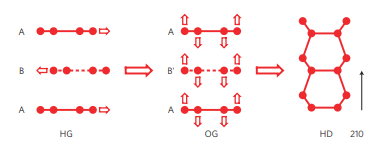
\includegraphics[width=0.7\columnwidth]{formlonsdaleite.png}
	\caption{ 	\label{lon}
		Formazione della lonsdaleite dalla grafite. 
		L'instabilità dei piani basali del reticolo HG provoca la formazione della HD.
	}
\end{figure}
Come si nota dalla fig \ref{lon}, l'instabilità della conformazione del reticolo HG determina la formazione di HD. Maggiori informazioni su tale processo si spiegano sul capitolo \ref{fif}.
La lonsdaleite però è stata ricavata anche da altri allotropi del carbonio, tra cui il $C_{60}$ sotto i 13-25 GPa e a 2600 K.
La lonsdaleite in verità può anche provenire dal diamante. Nel 2011 infatti fu sintetizzata da esso attraverso il suo surriscaldamento. Invece nel 1998 si eseguì il test di indentazione su una superficie diamantata utilizzando un indentatore diamantato e da tale processo si è ricavata la lonsdaleite. Essa in ogni caso viene osservata in piccole quantità all'interno dei cristalli di diamante, ma vi sono ancora numerosi problemi irrisolti riguardanti le sue peculiarità strutturali e sulla forma in cui appare. 
\section{Reticolo Cristallino}
\subsection{Struttura del reticolo}
La struttura cristallina esagonale della lonsdaleite conferisce alla cella unitaria la struttura in fig.\ref{lonsda},
\begin{figure}[h!] 
	\centering
	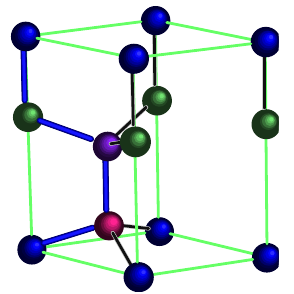
\includegraphics[width=0.5\columnwidth]{unitcelllonsda.png}
	\caption{ 	\label{lonsda}
		Struttura della cella unitaria della lonsdaleite. Per ognuna di esse si hanno quattro atomi, che in figura sono di quattro colori diversi.
	}
\end{figure}
avente 4 atomi per cella. I parametri reticolari sono pari ad $a = b = \SI{2.4834}{\angstrom}$ e $c = \SI{4.1354}{\angstrom}$, con gli atomi di C che occupano la posizione (0,33333, 0,66667, 0,06269), secondo il gruppo spaziale $D_{2h}^5$, lo stesso della grafite, ma con diverse posizioni atomiche nei siti reticolari.\\
\begin{figure}[h!] 
	\centering
	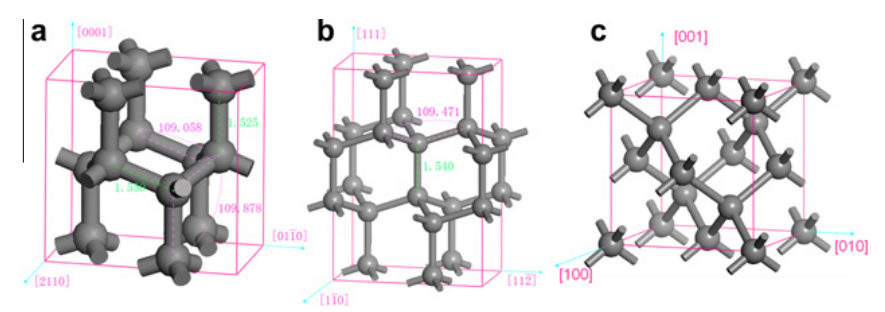
\includegraphics[width=0.8\columnwidth]{lonsdaleite.png}
	\caption{ 	\label{lonsdale}
		Differenza fra lonsdaleite e diamante. (a) cella di lonsdaleite rettangolare nel sistema di coordinate ortorombiche ridefinite per gli orientamenti [2 1 1 0], [0 1 1 0], [0 0 0 1] (b) cella rettangolare nel sistema di coordinate ortorombiche ridefinite per gli orientamenti di diamante [1 1 2], [1 1 0], [1 1 1]. (c) Cella del diamante nel sistema di coordinate ridefinito con gli orientamenti [1 0 0], [0 1 0], [0 0 1].
	}
\end{figure}
Dalla Figura \ref{lonsdale}, si può vedere che i tre assi cristallografici principali della lonsdaleite sono orientati lungo le direzioni [2 1 1 0], [0 1 1 0] e [0 0 0 1].
La forma della lonsdaleite è simile a quella del diamante, ad eccezione di uno spostamento laterale di uno dei due strati di carbonio, lungo la direzione [1 1 1]. Il vettore unitario lungo l'asse \textbf{c} per la lonsdaleite è $a_o \sqrt{3} = \SI{2,06}{ \angstrom}$, considerevolmente più piccolo della separazione interplanare di $\SI{3,35}{\angstrom}$ per la grafite.
\begin{figure}[h!] 
	\centering
	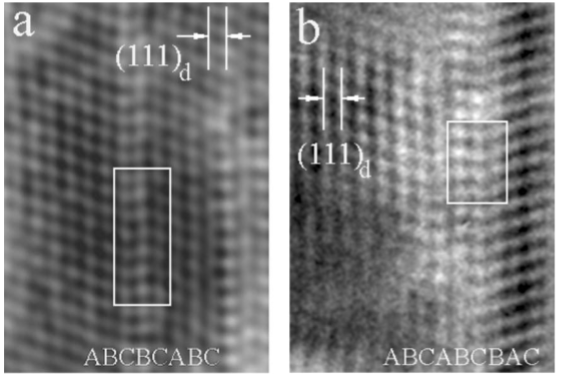
\includegraphics[width=0.8\columnwidth]{InfiltroLons.png}
	\caption{ 	\label{lonsdaleite}
		Immagini ad alta risoluzione del reticolo del diamante, asse di zona [110]. Gli errori di impilamento formano gli strati di lonsdaleite: (a) un singolo strato atomico A è stato rimosso dalla sequenza di strati ABCABCABC, formando una struttura CBC. Di conseguenza, l'interstrato di lonsdaleite è stato formato all'interno della struttura del diamante. (b) Abbiamo una struttura ABCABCBAC. Come mostrato, la sequenza di impilamento è specchiata, il che indica una formazione di struttura doppia. La struttura della lonsdaleite è data dalla composizione BCB.
	}
\end{figure}
Nel diamante la forma del reticolo cristallino rappresenta l'impilamento ABCABC, mentre nella lonsdaleite il reticolo cristallino rappresenta l'impilamento ABAB. Pertanto, i difetti di impilamento nel diamante sono identificati come strati del reticolo di lonsdaleite \ref{lonsdaleite} (immagine catturata da Kulnitskiy et al. \cite{Kulni}). La densità teorica della lonsdaleite è di $3,51 g/cm^3$, la stessa del diamante cubico. 
\subsection{Dispersione fononica}
Nel lavoro di Qian Wang et al. \cite{Qian}  si cominciò con l'ottimizzazione delle strutture cristalline di lonsdaleite, proseguendo quidi al calcolo della dispersione dei fononi (fig. \ref{ehehe}). 
\begin{figure}[h!] 
	\centering
	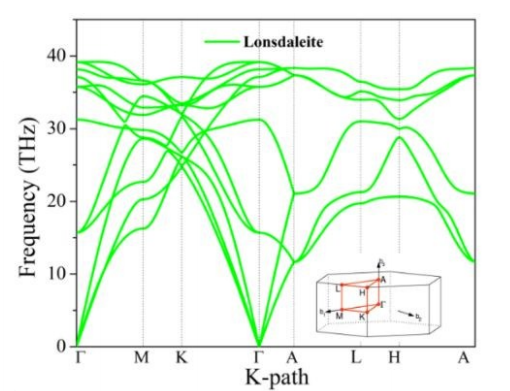
\includegraphics[width=0.7\columnwidth]{phonolonsda.png}
	\caption{ 	\label{ehehe}
		Dispersione fononica della lonsdaleite lungo i punti di alta simmetria. In basso a destra si ha una rappresentazione della prima zona di Brillouin con i punti principali di simmetria.
	}
\end{figure}
Il ramo acustico è piuttosto dispersivo, la velocità media del suono riscontrata è di $V_a = 13368 m/s$ determinata dalle proprietà elastiche, e risulta estremamente grande. Si noti che i rami ottici con la loro pendenza piuttosto ampia, sono in gran parte sovrapposti ai rami acustici. 
Tale andamento suggerisce che i fononi ottici della lonsdaleite possono immagazzinare una grande quantità di calore, e quindi danno contributi non trascurabili alla conducibilità termica $\kappa_L$ a causa della loro $V_g$ diversa da zero (velocità di gruppo dei fononi). Inoltre, a causa della presenza di più rami fononici (per via dei quattro atomi per cella primitiva), il sistema è più complesso.
\section{Proprietà fisiche e applicazioni possibili}
La zona centrale del diagramma di fase attorno a 18 GPa e 1.400 K  è stata attribuita ad una fase chiamata "diamante esagonale estraibile", che corrisponde alle condizioni in cui si genera la lonsdaleite. Essa risulta essere di grande interesse in quanto ha proprietà meccaniche potenzialmente superiori agli altri allotropi, anche del diamante, in resistenza a compressione, durezza e rigidità.\\
Nel lavoro di Quingkun et al. \cite{qing} sono stati attentamente calcolati matrice di rigidezza, modulo di Young (di rigidezza), modulo di compressibilità, resistenza alla compressione e resistenza alla trazione. 
Il modulo di compressibilità calcolato della lonsdaleite è 437,09 GPa, quasi uguale a 437,88 GPa del diamante. Questo ci suggerisce che la lonsdaleite ha la stessa capacità di resistere alla compressione uniforme del diamante. Inoltre, i componenti della matrice di rigidità C13, C23 per la lonsdaleite sono vicini allo zero, rispetto ai 50 GPa del C13 e del C23 per il diamante, simili a quelli nelle altre direzioni. Questo dimostra che lo sforzo e lo stress lungo l'orientamento [0 0 0 1] della lonsdaleite si discosta dallo stress lungo gli altri orientamenti perpendicolari a [0 0 0 1], e indica che la lonsdaleite offre migliore resistenza in una direzione.
La massima resistenza alla compressione della lonsdaleite raggiunta, cioè 727,16 GPa, è del $33,4\%$ superiore al valore corrispondente per il diamante, 545,09 GPa. Questi risultati indicano che la lonsdaleite potrebbe essere la sostanza naturale più dura presente sulla terra. 
In questo lavoro emerge anche che la lonsdaleite possiede le caratteristiche tipiche delle interazioni del legame $sp^3$, sebbene esistano differenze infinitesimali tra gli angoli dei legami della lonsdaleite e del diamante. In più presenta anche una struttura cristallina più ordinata. Le eccellenti proprietà meccaniche della lonsdaleite si attribuiscono dunque principalmente da due fonti: forte interazione $sp^3$ e una struttura cristallina più ordinata.\\

Tuttavia, queste proprietà eccezionali non sono state provate sperimentalmente a causa dell'incapacità di sintetizzare la lonsdaleite pura. È stato segnalato che si può formare durante la compressione statica della grafite, nel trattamento ad alta pressione e ad alta temperatura di polvere di diamante, grafite e carbonio amorfo; detonazione esplosiva e compressione shock di grafite e diamante; e deposizione chimica in fase vapore di gas di idrocarburi; tuttavia, in tutti i casi il prodotto di sintesi conteneva anche diamante, grafite o entrambi.
Nonostante i numerosi studi di diffrazione e spettroscopia, non sono stati riportati dati univoci che provano l'esistenza della lonsdaleite come materiale a se stante. 
Nel caso si riuscisse a sintetizzare la lonsdaleite nanopolicristallina, si prevede che la sua durezza superi significativamente i 200 GPa. Questa ricerca indica una nuova direzione per lo sviluppo di materiali superduri ad alte prestazioni e promettenti innovazioni sia nel settore della lavorazione delle macchine che in quello del lavoro ad alte pressioni.

\chapter{Fullereni}
\section{Generalità}
I fullereni furono scoperti nel 1985. Fu una scoperta così importante che scatenò l'interesse di ricercatori di ogni parte del mondo.
Un fullerene è una molecola caratterizzata dalla forma di una sfera cava, di un ellissoide o di forma tubulare. In base alla forma essi hanno caratteristiche, utilizzi e proprietà completamente differenti. Essi sono suddivisibili in due macrocategorie che andremo ad analizzare: la prima comprende fullereni di forma sferoidale o ellissoidale. In tale categoria rientra il \textit{Buckminster fullerene} ($C_{60}$) o \textit{"bucky ball"}, avente una struttura sferica chiusa composta da circa venti anelli esagonali e dodici pentagonali; ciascun atomo di carbonio è in ibridizzazione $sp^2$. Le altre possibili strutture di fullereni sferoidali cambiano al variare del numero di atomi di carbonio. Se tale numero lo permette infatti si creano degli anelli esagonali, dunque tali molecole differiscono nel numero di anelli esagonali presenti. La $C_{70}$ sembra simile a una palla da rugby (fig. \ref{c60}) ed il $C_{120}$ prende una forma di manubrio. Si hanno poi le molecole $C_{20}$, $C_{26}, C_{28}, C_{32}, C_{50}, C_{70}, C_{76}, C_{78}$. Il fullerene $C_{20}$ è il più piccolo possibile.\\
\begin{figure}[h!] 
	\centering
	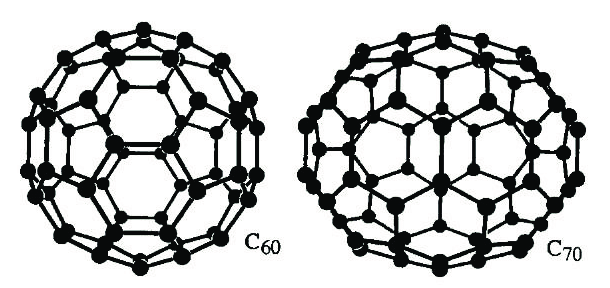
\includegraphics[width=0.6\columnwidth]{aaaaaa.png}
	\caption{ 	\label{c60}
		Fullerene $C_{60}$ (a destra) e $C_{70}$ (a sinistra).
	}
\end{figure}
La seconda categoria è composta da fullereni di forma tubulare, detti \textit{nanotubi di carbonio}, o \textit{"Carbon NanoTubes"}. Un CNT è un foglio di grafene arrotolato a forma di cilindro, esso ha quindi lo spessore di un atomo. Sono stati costruiti CNT con un rapporto lunghezza-diametro di $132000000:1$, che è significativamente più alto di qualsiasi altro materiale. Ve ne sono di vario tipo: nanotubi a parete singola, nanotubi a parete multipla, Graphenated CNT \ref{swmww} (nanotubi di carbonio con struttura ibrida in cui la grafite a lamelle è cresciuta lungo la lunghezza di un CNT a più pareti allineate), extreme CNTs (la tipologia di nanutubo più corto), nanotubi toroidali\ref{pea}, peapod CNTs\ref{pea}, Cup-stacked CNTs \ref{swmww}, Carbon megatubes \ref{meg}.
Altri tipi di fullerene sono i Carbon onions, ed i Bucky ball clusters\ref{ONYO}.
In tale resoconto si prenderanno in esame solo i fullereni più interessanti per proprietà e struttura, ma anche i più importanti in applicazioni pratiche. 
\begin{figure} [h!]
	\centering
	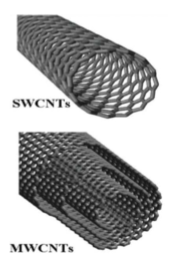
\includegraphics[width=.4\textwidth]{SWMW.png}\hfil
	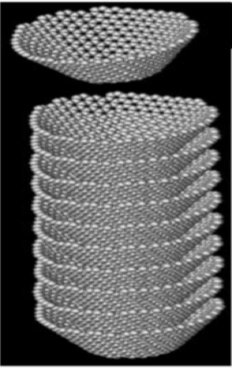
\includegraphics[width=.4\textwidth]{cupstacked.png}
	
	\caption{\textit{a sinistra}, nanotubi a parete singola (sopra) e parete multipla (sotto). \textit{a destra},  Cupstaked CNT, nanofibre di carbonio lunghe e dritte, con un nucleo cavo, impilate una sopra l'altra.}\label{swmww}
\end{figure}
\begin{figure}[h!]
	\centering
	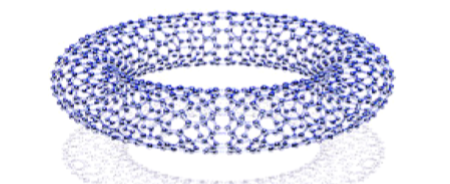
\includegraphics[width=.49\textwidth]{torus.png}\hfil
	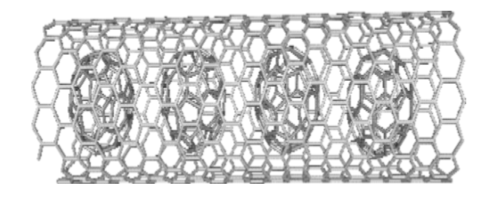
\includegraphics[width=.49\textwidth]{peapod.png}
	
	\caption{\textit{a sinistra}, nanotubo toroidale; \textit{a destra}, peapod CNT, costituito da fullereni sferoidali incapsulati all'interno di un nanotubo di carbonio. }\label{pea}
\end{figure}

\begin{figure}[h!] 
	\centering
	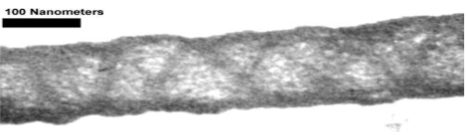
\includegraphics[width=0.6\columnwidth]{megatube.png}
	\caption{ 	\label{meg}
	Carbon megatube, del diametro di circa 100 nm.}
\end{figure}
\begin{figure}[h!]
	\centering
	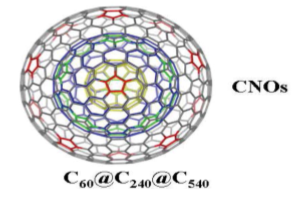
\includegraphics[width=.49\textwidth]{onion.png}\hfil
	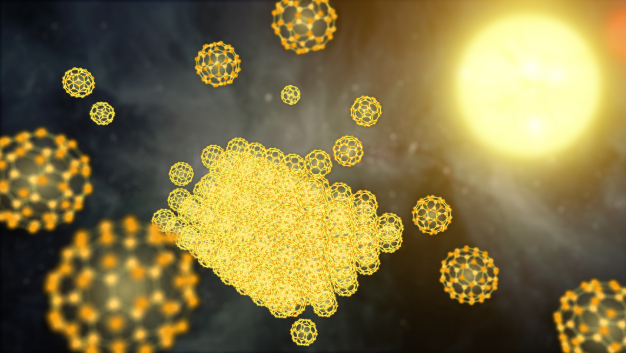
\includegraphics[width=.49\textwidth]{buckyball.png}
	
	\caption{\textit{a sinistra}, Carbon onion. Si tratta di fullereni concentrici, formanti una struttura a multi-layer. Accade principalmente in caso di masse elevate; \textit{a destra}, Bucky Ball cluster. }\label{ONYO}
\end{figure}

\newpage
\section{Scoperta e sintetizzazione}
\subsection{Scoperta}
Il primo ad essere stato scoperto fu il fullerene $C_{60}$, esso è infatti presente in natura in piccole quantità. La sua recente sintesi è da attribuirsi nel 1985 da parte del fisico H. W. Kroto, che studiò alcune molecole organiche nello spazio con esattamente 60 atomi di carbonio trovate vicino a varie stelle giganti rosse. Per questo, Kroto ha collaborato con Smalley e Curl per ricreare le condizioni in laboratorio e formare molecole $C_{60}$ mediante la vaporizzazione laser della grafite. Dopo tale esperimento si scoprì analizzando le molecole di $C_{60}$  che erano fatte di anelli pentagonali ed esagonali che sono simili nella struttura alla grafite, molto simile alla cupola geodetica progettata dall'architetto Buckminster Fuller. Il nome che fu attribuito alla molecola dunque è in onore dell'architetto.

La scoperta dei nanotubi di carbonio è stata anche più recente: nel 1991 il fisico Ijiyama di NEC Japan ha annunciato la sintesi dei nanotubi di carbonio (CNT). Nei suoi esperimenti di ionizzazione di gas con elettrodi fatti di grafite, insieme alle particelle di fuliggine raccolte c'erano alcune strutture sottili a forma di tubo. Grazie ad un'analisi attenta si comprese che si trattava di nanotubi di carbonio (CNTs). Questi nanotubi a parete singola sono tubi lunghi interamente fatti di carbonio, sostanzialmente costituiti da un foglio di grafite che viene avvolto a forma di tubo, con un diametro di qualche nanometro e una lunghezza di pochi micron. 
Secondo la NASA, nel 2010 alcuni fullereni sono stati scoperti in una nuvola di polvere cosmica simile a una stella lontana di 6.500 anni luce di distanza e si sospetta che i fullereni esistano nello spazio fin dall'era primordiale, nei buchi neri delle nostre galassie. Infine, l'esistenza dei fullereni nello spazio è stata confermata in modo inequivocabile nel 2014 da alcuni scienziati canadesi. 

\subsection{Sintetizzazione}
I fullereni possono essere sintetizzati in laboratorio in una grande varietà di modi, tutti con la generazione di un vapore o plasma ricco di carbonio. Tutti i metodi attuali di sintesi di fullereni producono principalmente $C_{60}$ e $C_{70}$, queste molecole sono ora ordinariamente isolate in quantità copiose e sono disponibili commercialmente. Anche i fullereni di massa più elevata possono essere realizzati e isolati, sebbene in quantità sostanzialmente ridotte. \\

I primi approcci alla sintesi di fullereni utilizzavano tecniche di vaporizzazione laser, che producevano solo quantità microscopiche di fullereni che, nella fase gassosa, venivano studiati in un apparato a fasci molecolari. Usando queste tecniche, i primi esperimenti di Kroto, Smalley et al. nel 1985 suscitarono un grande interesse nella comunità di ricerca per riprodurre e isolare quantità macroscopiche di fullereni. La svolta avvenne nel 1990 quando Kritschmer et al. scoprirono che le barre di carbonio, se riscaldate in un'atmosfera di elio a circa $200 mmHg$, generano una discreta quantità di fullereni, assieme alla fuliggine. Devono quindi essere estratti da essa e successivamente purificati. Questo risulta essere attualmente il metodo più efficiente per produrre i fullereni. \\
Se si desidera una soluzione di fullerene purissima, è necessario eseguire una fase finale di purificazione chimica. Per quanto riguarda la separazione dei fullereni di massa elevata, si ritiene che come sottoprodotto della preparazione di grandi quantità di $C_{60}$ e $C_{70}$ in commercio, saranno disponibili quantità minori di fullereni di massa più elevata. \\

Per quanto riguarda i nanotubi vi sono una quantità elevata di tipologie di sintetizzazione, in quanto essi sono largamente richiesti per via delle loro ottime proprietà fisiche. Sono state sviluppate due strategie principali di produzione: (1) grow-in-place e (2) grow-then-place.\\
Il primo approccio consiste principalmente nel rendere il campione disponibile nei quartieri in cui i CNT saranno sintetizzati. La sintesi viene tipicamente condotta utilizzando approcci CVD (chermical vapor deposition). La tecnica CVD è uno dei metodi migliori per produrre CNT con forma ben definita, dimensioni e proprietà fisiche che si desiderano ottenere.  Esso prevede l'esposizione del substrato a uno o più precursori volatili, che si decompongono o reagiscono sulla superficie del substrato per fornire il deposito ricercato. I sottoprodotti volatili vengono prodotti anche durante questo processo che può essere separato dal gas attraverso la camera di reazione. Oggigiorno, il processo CVD è il metodo comunemente usato per la sintesi dei CNT.\\
Il secondo approccio prevede prima la sintesi di nanotubi di carbonio e successivamente il loro spostamento verso il luogo di destinazione. L' Ablazione laser e ionizzazione del gas sono storicamente i due principali approcci applicati per produrre nanotubi con questo approccio.
Il primo si esegue con lo stesso apparato per la sintetizzazione del $C_ {60}$ di Kroto et al., e coinvolge la pressurizzazione di atomi di carbonio prodotti da fonti solide di carbonio. La temperatura richiesta in questo esperimento era $3000-4000 ^\circ C$ che è abbastanza vicino alla temperatura di fusione della grafite.
Il secondo è lo stesso metodo di produzione del $C_ {60}$, in questo processo il prodotto è ottenuto come miscela di SWCNT e MWCNT insieme ad altri componenti.
Successivamente alla loro sintesi, i nanotubi si trasferiscono nelle regioni preselezionate del substrato bersaglio. Solo pochi sistemi hanno mostrato risultati eccezionali, come ad esempio la deposizione da una soluzione che utilizza campi elettrici alternati, o tecniche litografiche.
\section{Reticolo cristallino}
\subsection{Caratteristiche del reticolo nei fullereni sferoidali}
L'ibridazione dei legami dei fullereni non è uguale per ogni legame, ha caratteristiche variabili a seconda del numero di atomi di carbonio nella molecola. Questo numero varia da venti per il $C_{20}$ (il primo fullerene stabile geometricamente) fino ad infinito per la grafite (che potrebbe essere considerata come il caso estremo di tutte le possibili strutture fullereniche). Ciò determina la dimensione della molecola, così come la determina l'angolo di piramidalizzazione della struttura (l'angolo comune ai tre legami $\sigma$ tipici dell'$sp^3$). Il numero di atomi di carbonio, l'angolo di piramidalizzazione ($\theta_{\sigma\pi}-90^\circ$) e la natura dell'ibridazione sono correlati; questa relazione è riportata in Fig.\ref{dia}, in questo caso abbiamo in ordinata il parametro \textit{s character}, un parametro che ci informa di quanto contibuisce il legame di tipo $\sigma$ nell'ibridazione.
\begin{figure}[h!] 
	\centering
	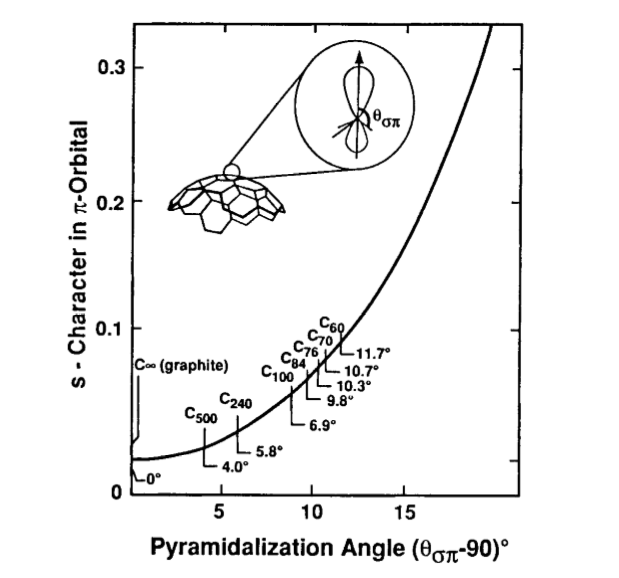
\includegraphics[width=0.7\columnwidth]{anglediag.png}
	\caption{ 	\label{dia}
		Diagramma che spiega come l'angolo di piramidalizzazione e l' \textit{s character} sono correlati.
	}
\end{figure}
Le lunghezze dei legami dei fullereni per gli anelli a cinque e sei atomi sono $r_{fs}=0,145 \pm 0,0015 nm$ e $r_{ss}0,140 \pm 0,0015 nm$. \\
Vediamo sommariamente le caratteristiche strutturali dei reticoli delle bukyball:
\begin{itemize}
\item $C_{20}$ : è la struttura più semplice, composta da dodici pentagoni senza alcun esagono, con un angolo di piramide di $18^\circ$. Tutti i suoi atomi hanno configurazione $sp^3$, ed è termodinamicamente instabile.
\item $C_{60}$ : Il primo fullerene stabile e il primo a essere scoperto è il $C_ {60}$. È la molecola predominante in natura essendo la più stabile, con sessanta atomi di carbonio disposti in modo da formare venti esagoni e dodici pentagoni, dandogli l'aspetto di un pallone da calcio. Ogni esagono è collegato ad un pentagono e ad un altro esagono, quindi ogni atomo di carbonio è condiviso da un pentagono e da due esagoni. La sua ibridazione è parzialmente $sp^3$ e parzialmente $sp^2$, con un angolo di piramide di $11,6^\circ$, mostrato schematicamente in Fig. \ref{c60}\textit{(sinistra)}. Il $C_{60}$ ha un diametro calcolato di $d=0,710 \pm 0,007 nm$. È intensamente viola in solventi apolari.
\item $C_{70}$ e fullereni a più di 70 atomi di carbonio: il $C_{70}$, è il secondo fullerene più abbondante. Assomiglia ad una palla da rugby \ref{c60}\textit{(destra)} e in soluzione è di colore arancio-rosso intenso. Il $C_ {76}$ è chirale con una struttura composta da una disposizione a spirale di pentagoni ed esagoni. Ha un colore giallo-verde brillante in soluzione. Il $C_ {78}$, è marrone o giallo dorato e il $C_{84}$ è verde oliva.
\end{itemize}

\subsection{Formazione del reticolo cristallino di un fullerene}
Come descritto da Smalley, la formazione di un fullerene segue un "efficiente meccanismo di auto-assemblaggio di una struttura architettonicamente utile su scala nanometrica". \\

Un modello del meccanismo di formazione dei fullereni è basato sulla regola del "Pentagono isolato"; essa stabilisce che tale struttura geometrica deve soddisfare i seguenti tre criteri: (a) deve essere fatta solo di esagoni e pentagoni, (b) deve avere dodici pentagoni, e (c) non deve includere pentagoni adiacenti. Questo ultimo criterio è richiesto anche dal punto di vista termodinamico poiché la fusione di due pentagoni vicini non è favorevole energeticamente, dunque le strutture di carbonio con pentagoni adiacenti sono instabili. \\
Il $C_{60}$, è il primo fullerene che evita i pentagoni confinanti ed è la più stabile e simmetrica di tutte le molecole di fullerene stabili. Le strutture più piccole, come il $C_{20}$, non possono essere stabili poiché conterrebbero pentagoni confinanti. \\
Di seguito è riportato il processo generale di formazione di un fullerene. In prima analisi si pensava che la molecola inizialmente si presentasse come una rete di grafite che aggiunge atomi di carbonio a formare pentagoni provocando l'arricciamento del foglio di grafite che arriva a formare una sfera geodetica. Un meccanismo più probabile è la formazione mediante l'aggregazione di piccoli radicali liberi di carbonio. Ciò si verifica quando la grafite viene vaporizzata a temperature molto elevate. I fogli di grafite liberi condensano nel vapore, ma non hanno energia sufficiente per formare legami e la tendenza fisica a raggiungere il livello di energia più basso li induce ad arricciarsi e creare la struttura del fullerene. Un'ipotetica sequenza di crescita è mostrata in Fig. \ref{gro}. \\
\begin{figure}[h!] 
	\centering
	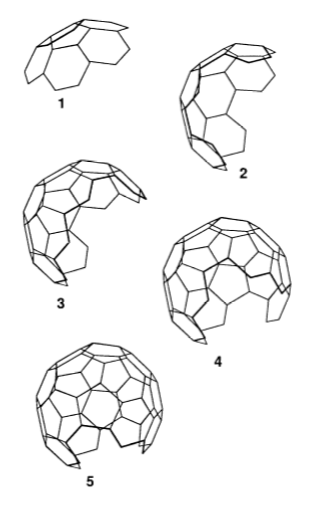
\includegraphics[width=0.35\columnwidth]{growth.png}
	\caption{ 	\label{gro}
		Una possibile sequenza che descrive la crescita di un fullerene $C_{60}$.
	}
\end{figure}
Ogni atomo di carbonio nel $C_{60}$ ha due legami singoli lungo i lati adiacenti di un pentagono e un doppio legame tra due esagoni adiacenti. Se questi legami fossero complanari, sarebbero molto simili al legame $sp^2$ nella grafite. La superficie del $C_{60}$ rende gli orbitali $sp^2$ ibridi con gli $sp^3$: ciò causa un accorciamento dei legami doppi, che raggiungono dimensioni di circa $\SI{1,40}\angstrom$ e un allungamento legami singoli afino a $\SI{1,46}\angstrom$. Tale modifica strutturale negli anelli esagonali della molecola $C_{60}$ influenza fortemente la struttura elettronica.\\

Si approfondirà solo il $C_{60}$ molecolare, il più abbondante in natura.
\subsection{Reticolo cristallino del $C_{60}$ molecolare}
Nello stato solido, le molecole $C_{60}$ cristallizzano in una struttura cubica, con una costante reticolare di $a=\SI{14.17}{\angstrom}$, una distanza fra primi vicini $r_{C_ {60} -C_ {60} }=\SI{10,02}{\angstrom}$ e una densità di $\rho=1,72 g / cm^3$. Mentre le molecole $C_ {60}$ sono quasi incomprimibili, il solido molecolare è piuttosto comprimibile. Pertanto, sotto la pressione idrostatica, si prevede che la densità di massa del solido $C_{60}$ dovrebbe aumentare in modo significativo. Un diagramma di fase proposto per $C_ {60}$ è mostrato in Fig. \ref{difull}.
\begin{figure}[h!] 
	\centering
	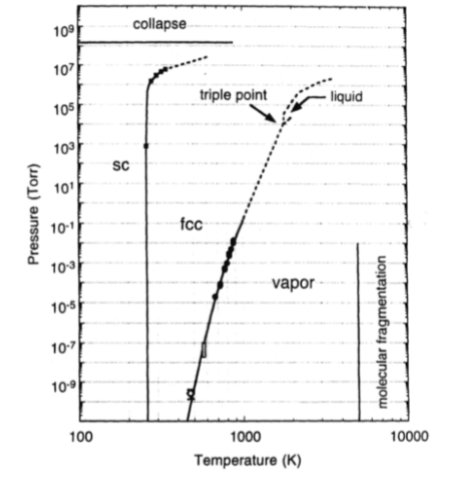
\includegraphics[width=0.7\columnwidth]{diagfulle.png}
	\caption{ 	\label{difull}
		Diagramma di fase per il $C_{60}$ molecolare.
	}
\end{figure}
A temperatura ambiente, sono state osservate molecole di $C_ {60}$ in forma solida grazie alla risonanza magnetica nucleare (NMR). Le molecole di fullerene sono disposte su un reticolo fcc, rappresentato in Fig.\ref{fcc}. Si può scegliere fra due tipi di celle unitarie, caratterizzate da una o quattro molecole per cella unitaria.
\begin{figure}[h!]
	\centering
	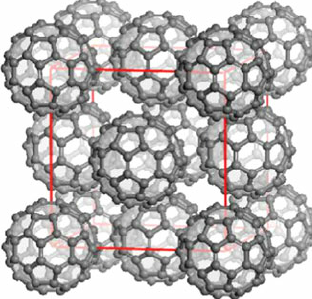
\includegraphics[width=.49\textwidth]{cubicfullerene.png}\hfil
	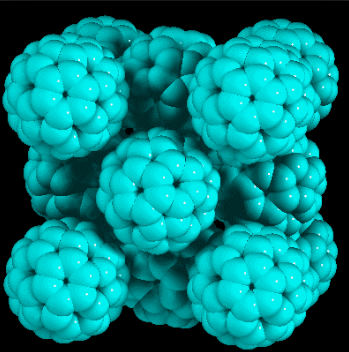
\includegraphics[width=.49\textwidth]{cubicfullfigo.png}
	
	\caption{ Struttura del fullerene $C_{60}$ molecolare del tipo fcc. }\label{fcc}
\end{figure}

Tale struttura cristallina persiste fino alla temperatura di $T_1=261K$ in cui si verifica una transizione verso la forma simple cube (sc).
Le lunghezze dei legami $C-C$ nella fase solida sono essenzialmente le stesse della fase gassosa. 
Rispetto alle altre forme allotropiche del carbonio, il solido $C_ {60}$ è relativamente comprimibile, con una compressibilità di volume a temperatura costante di $6,9 \cdot 10^{-12} cm^2 / dyn$, circa tre volte più grande di quella della grafite, poiché la nube di Van der Waals attorno alle molecole di $C_ {60}$ può essere compressa facilmente essendo la struttura in tre dimensioni piuttosto che in una dimensione, come nel caso della grafite. 
\subsection{Modi vibrazionali del $C_{60}$ molecolare}
Poiché il solido $C_{60}$ è quasi un solido molecolare ideale, i suoi modi vibrazionali possono essere suddivisi in due classi: vibrazioni intermolecolari (o modi di reticolo) e vibrazioni intramolecolari (o semplicemente modi "molecolari"). Tali modi possono essere ulteriormente suddivisi in tre sottoclassi: modi acustici, ottici e le librazioni. I primi due sono dei modi intermolecolari di cui dispongono tutti i solidi atomici: hanno tre modi acustici e tre modi ottici, legati alle tre dimensioni spaziali. Per tutti i solidi molecolari, si presenta una terza sottoclasse di modi detti di "librazione", facenti parte dei modi molecolari. Esse derivano dal momento di inerzia della molecola $C_{60}$ e implicano una rotazione attorno all'asse delle molecole stesse. Le frequenze dei modi di librazione sono piuttosto basse perché le molecole sono fra loro debolmente accoppiate e anche perché il momento di inerzia delle molecole di fullerene è grande.\\

Si possono determinare i modi traslazionali utilizzando due cristalli singoli liberi, con un volume di scattering di $3 mm^3$. I risultati sono mostrati in figura. \ref{pho}.
\begin{figure}[h!] 
	\centering
	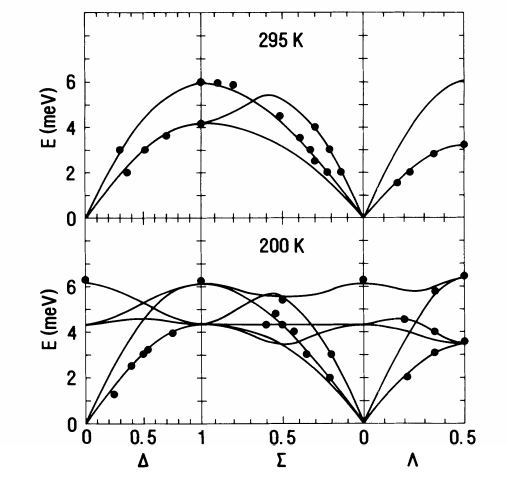
\includegraphics[width=0.7\columnwidth]{phononc60.png}
	\caption{ 	\label{pho}
		Modi traslazionali per il $C_{60}$ molecolare. Le linee continue sono le funzioni calcolate teoricamente, i punti sono i valori sperimentali campionati.
	}
\end{figure}
Le velocità di fase dei  rami trasversali e longitudinali acustici (velocità del suono) sono state recentemente calcolate sperimentalmente, e sono rispettivamente $v_{exp.ft}=3.38 \cdot 10^3 m/s$    e   $v_{exp.fl}=1.57 \cdot 10^3 m/s$, nella direzione $ [111] $, mentre quelle teoriche erano $v_{ft}=2.21 \cdot 10^3 m/s$    e   $v_{fl}=4.16 \cdot 10^3 m/s$, rispettivamente.
La figura mostra la dispersione calcolata per i modi traslazionali (linee), ed i modi acustici (linee che emergono dal punto 0), a due temperature diverse, sopra e sotto la temperatura di transizione da sc a fcc, ossia $T=261 K$.
Le linee del grafico sono il risultato di un fit eseguito in base al modello di Born-von Kràman che prevede l'azione di una forza costante a due parametri, ossia le forze longitudinali costanti che derivano dall'azione dei due primi vicini (NN). Un fit di qualità elevata può essere ottenuto assumendo che le forze dell'azione dei due primi vicini possano essere ricondotte ad un unico tensore che richiede tre parametri per effettuare il fit. Per eseguire i calcoli in maniera più semplice si assume che il reticolo sia di tipo fcc anche per il campionamento a $T=200K$, in tal modo si ignora la perdita di simmetria causata dal passaggio da fcc a sc.
Il buon accordo tra il modello e l'esperimento indica che questa ipotesi è ragionevole per i modi traslazionali. 
La forma generale delle curve di dispersione è simile a quella trovata per i gas nobili allo stato solido, il che non ci sorprende in quanto il $C_{60}$ ha simmetria sferica, ed ha legami molto simili ad essi.
\begin{figure}[h!] 
	\centering
	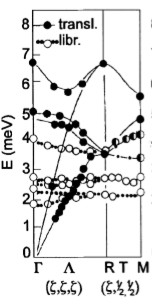
\includegraphics[width=0.25\columnwidth]{librational.png}
	\caption{ 	\label{fig:lib}
		Diagramma dei modi librazionali.
	}
\end{figure}
I modi in Fig. \ref{fig:lib} rappresentano modi librazionali e traslazionali. Essi sono indicati rispettivamente dai cerchi vuoti e pieni. Come si può vedere, la dispersione dei ramo acustico è sufficientemente ampia da sovrapporsi a tutti i rami ottici e mostra una frequenza massima di $6,7 meV (55 cm^{-1})$. Inoltre, i modi librazionali sono i quattro rami ottici più bassi osservati, con frequenze inferiori a quelle che ci si aspetterebbe da un'analisi di misurazioni di calore specifico. Si nota poi che questi modi librazionali non mostrano quasi nessuna dispersione. I due rami ottici superiori, che presentano frequenze in zona centrale di $5 meV$ e $6,7 meV$, sono in ottimo accordo con le frequenze di modo osservate rispettivamente a $41 cm^{-1}$ di $5,1 meV$ e a $55 cm^{-1}$ di $6,8 meV$ a $T=1.5K$.

\subsection{Reticolo cristallino dei nanotubi di carbonio}
I nanotubi di carbonio e i fullereni hanno una serie di caratteristiche comuni, ma anche molte differenze. Concentriamo l'attenzione sui tubuli a parete singola. Essi sono di forma cilindrica, matematicamente di lunghezza infinita o con "cappucci" a ciascuna estremità, in modo che i due "cappucci", se uniti, formano un fullerene sferico. Formalmente, la parte cilindrica del tubulo consiste in un singolo foglio di grafene, arrotolato a formare un cilindro.
\begin{figure}[h!] 
	\centering
	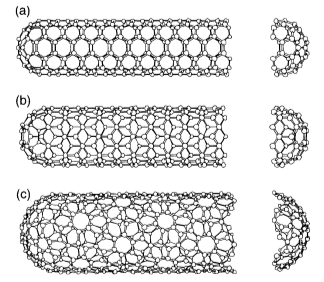
\includegraphics[width=0.55\columnwidth]{nanotube.png}
	\caption{ 	\label{bohh}
		In figura si riportano tre dipi differenti di nanotubi di carbonio: (a)-nanotubo "armchair"; (b)-nanotubo "zig zag"; (c)-nanotubo "chirale".
	}
\end{figure}
In fig. \ref{bohh} vediamo degli esempi di nanotubi di carbonio a parete singola che hanno come base il fullerene $C_{60}$. Bisecando tale molecola all'equatore e unendo i due emisferi risultanti con un tubo cilindrico  dello stesso diametro si ottiene un tubulo. Se la molecola di $C_{60}$ è divisa in due da un asse a cinque pieghe si forma il tubulo "armchair" in fig. \ref{bohh}-(a).  Se la molecola di $C_{60}$ viene tagliata su un asse a tre pieghe, si crea il tubulo "a zigzag" in Fig.\ref{bohh}-(b).
\begin{figure}[h!]
	\centering
	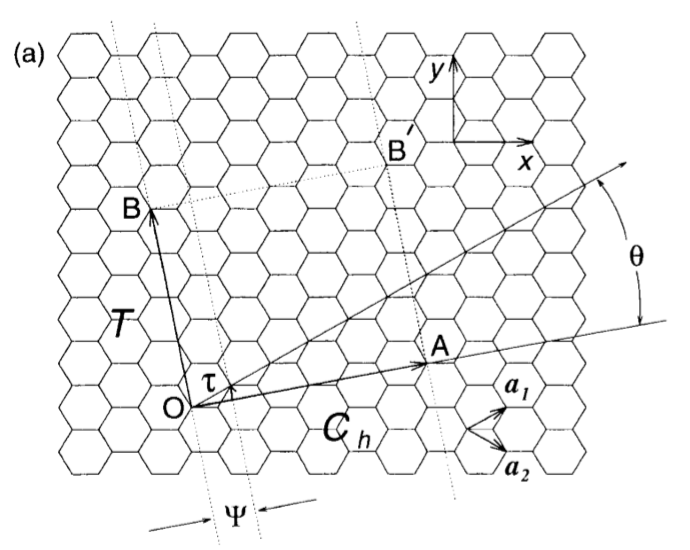
\includegraphics[width=.49\textwidth]{chirl.png}\hfil
	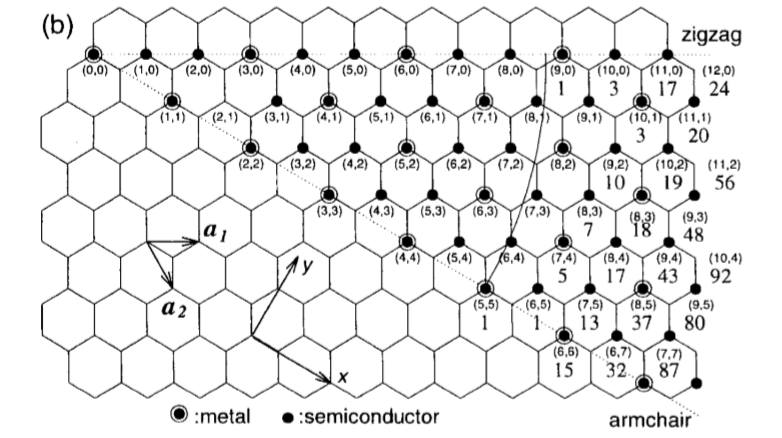
\includegraphics[width=.49\textwidth]{chirl1.png}
	
	\caption{ 
		(a)-il vettore chirale OA è definito sul reticolo esagonale di atomi di carbonio dai vettori unitari $a_l$ e $a_2$ e l'angolo chirale $\theta$ rispetto all'asse a zigzag; (b)-Si hanno i possibili tubuli specificati dalle coppie di interi (n,m), che saranno a zig-zag, armchair o tubuli chirali. Sotto ogni coppia di interi (n,m) è elencato il numero di cappucci possibili per i tubuli di carbonio indicato da (n,m). 
		I punti circondati denotano tubuli metallici mentre i punti piccoli denotano tubuli semiconduttori. }\label{fig:chirale}
\end{figure}
Oltre ai tubuli armchair e ai tubuli a zigzag, esistono un gran numero di nanotubi di carbonio, e variano in base all'avvitamento lungo l'asse di simmetria del tubulo ed in base agli svariati tipi di cappucci semisferici. Tali parametri possono essere rappresentati matematicamente in termini di diametro tubulare $d_t$ e angolo chirale $\theta$, che sono mostrati in Fig. \ref{fig:chirale}-(a), con l'espressione per il vettore chirale OA che indicheremo con $C_h$:
\begin{equation} \label{ehe}
C_h=n\cdot a_1 + m \cdot a_2
\end{equation}
In Fig. $\ref{fig:chirale}-(a)$, il vettore $C_h$ collega due siti cristallograficamente equivalenti O e A su un foglio di grafene bidimensionale (2D) in cui un atomo di carbonio si trova in corrispondenza di ciascun vertice della struttura a nido d'ape. Si noti in figura l'angolo chirale $\theta$ del nanotubo rispetto alla direzione a zigzag ($\theta = 0^\circ$) e i vettori unitari $a_1$ e $a_2$ del reticolo esagonale. Il tubulo armchair in Fig.$\ref{bohh}-(a)$
corrisponde a $\theta= 30^\circ$, per come è stato costruito. Un insieme di possibili vettori chirali può essere specificato dall'Eq. \ref{ehe}  in termini di coppie di interi (n,m), e questo insieme è mostrato in Fig.$\ref{fig:chirale}-(b)$. Ogni coppia di interi (n,m) definisce un modo diverso di arrotolare il foglio di grafene per formare un nanotubo di carbonio.
Il cilindro che collega i due cappucci semisferici è formato sovrapponendo le due estremità OA del vettore $C_h$. La giunzione del cilindro viene realizzata unendo la linea AB' alla linea parallela OB, dove le linee OB e AB' sono perpendicolari al vettore $C_h$ a ciascuna estremità. Il tubulo chirale così generato non subisce delle distorsioni negli angoli che si trovano fra i legami causate dalla curvatura cilindrica del tubulo. Le differenze nell'angolo chirale $\theta$ e nel diametro del tubulo $d_t$ danno origine a differenze nelle proprietà dei vari nonotubi di carbonio. Nella notazione (n, m), i vettori (n,0) denotano tubuli a zigzag e i vettori (n,n) denotano tubuli armchair; e maggiore è il valore di n, maggiore è il diametro del tubulo. Entrambi i nanotubi (n,0) e (n,n) hanno un'alta simmetria. Tutti gli altri vettori (n,m) corrispondono a tubuli chirali. 
In termini di numeri interi (n,m), il diametro del tubulo $d_t$ è dato da:

\begin{equation}
d_t = C_h/\pi = \sqrt{3}a_{c-c}\frac{(m^2 + mn + n^2)^{l/2}}{\pi}
\end{equation}
dove $a_{c-c}$ è la distanza fra due primi vicini, $C_h$ è la lunghezza del vettore chirale.
L'angolo chirale $\theta$ è dato da:
\begin{equation}
\theta = tan^{-1}[\frac{\sqrt{3}m}{(m + 2n)}].
\end{equation}

\subsection{Dispersione fononica nei nanotubi di carbonio}
Le relazioni di dispersione dei fononi per un nanotubo di carbonio dipendono dagli indici (n,m), o equivalentemente dal diametro del tubulo e dalla chiralità.
\begin{figure}[h!] 
	\centering
	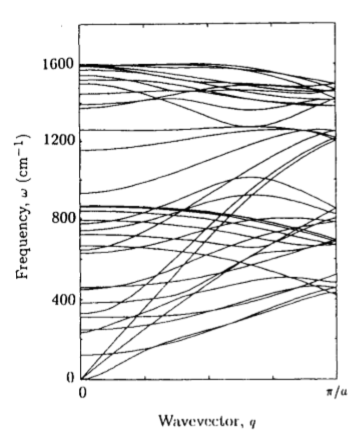
\includegraphics[width=0.55\columnwidth]{phononnanotubes.png}
	\caption{ 	\label{boom}
		Diagramma contenente le 36 relazioni di dispersione fononica 
	}
\end{figure}
Come esempio di un nanotubo di carbonio, il tubulo armchair (5,5) ha N = 10 atomi e 60 gradi di libertà per una cella unitaria unidimensionale, 12 rami fononici non degeneri, 24 rami fononici doppiamente degeneri, quindi vi sono 36 rami distinti.
Si mostrano di seguito le 36 relazioni di dispersione dei fononi per i nanotubi di carbonio nella fig.\ref{boom}, (corrispondente al tubulo con cappuccio semisferico di $C_{60}$).
Le relazioni di dispersione dei fononi, simili a quelle mostrate nella figura per il tubulo armchair (n,m) = (5,5), sono state calcolate anche per vari tubuli a zigzag e tubuli chirali. In generale, le relazioni di dispersione avranno molti più rami di quelli mostrati in Figura, a causa delle dimensioni maggiori della cella unitaria 1D per un nanotubo generale (n,m). Negli esperimenti che coinvolgono le relazioni di dispersione fononiche per i nanotubi di carbonio, le misurazioni sono fatte su una moltitudine di nanotubi, ciascuno con i propri indici (n,m). Se le misurazioni vengono fatte con l'ausilio della spettroscopia, allora gli spettri osservati saranno molto simili fra nanotubi differenti.

\section{Proprietà fisiche e applicazioni}
\subsection{Proprietà fisiche del $C_{60}$}
Gli aggregati di $C_ {60}$ sono considerati la più morbida delle fasi solide del carbonio. Tuttavia, se compressi a meno del $70\%$ del suo volume originale, potrebbero essere più duri del diamante. Hanno un'elevata resistenza all'impatto e resilienza. Risultano avere anche un alto potere lubrificante poiché le molecole sono legate dalle forze di Van der Waals lungo tutti i piani, e ciò consente alle molecole di scivolare facilmente l'una sull'altra  similmente ai piani di tipo ABAB dei cristalli di grafite.
Gli aggregati hanno una struttura a microfori con uno spessore di $1,19 - 1,26 nm$ e un'area superficiale interna relativamente alta ($131,9 m^2/g$).
Il $C_{60}$ è un semiconduttore a band-gap diretta, ossia quando il massimo della banda di valenza si ha per lo stesso k per il quale si ha il minimo della banda, similmente all'arseniuro di gallio. Tuttavia, le sue proprietà semiconduttive devono ancora essere determinate. 
La rapida compressione del $C_{60}$ in polvere a più di $150 atm$ in meno di un secondo causa un collasso dei fullereni e la formazione del diamante policristallino in una matrice di carbonio amorfo. Perciò, i fullereni sono la prima fase nota del carbonio che si trasforma in diamante a temperatura ambiente. \\ 
Per quanto riguarda la reattività chimica, sebbene la molecola sia stabile dal punto di vista fisico, ha un'elevata affinità elettronica ed è reattiva chimicamente, specialmente con i radicali liberi. I fullereni sono strutture aromatiche e si dissolvono facilmente nel benzene e in altri solventi aromatici. Si ossidano lentamente in una miscela di acido solforico e nitrico concentrato a temperature superiori a $50^\circ C$. In ossigeno puro il $C_{60}$ inizia a sublimare a $350^\circ C$ e si infiamma a $365^\circ C$.
La prima osservazione di superconduttività nel $C_{60}$ drogato ha attirato molta attenzione a causa della temperatura di transizione $T_C$ relativamente alta osservata, la prima osservazione è stata nel $K_3C_{60}$ drogato con metallo alcalino, con una $T_C=18 K$. Da allora la superconduttività dei fullereni drogati è rimasta un campo di ricerca molto attivo, poiché sono stati scoperti nuovi materiali superconduttori di fullerene e sono stati fatti tentativi per comprendere gli aspetti insoliti della superconduttività in questi materiali e il meccanismo di appaiamento per gli elettroni. Al momento attuale, la superconduttività è stata riportata solo per i solidi a base di $C_{60}$, sebbene le proprietà di trasporto fino a 1 K siano state misurate anche su $C_ {70}$ drogati con metalli alcalini e forse anche su fullereni di massa più elevata.

\subsection{Applicazioni del $C_{60}$}
Le proprietà di assorbimento nello stato di tripletto eccitato danno luogo a dispositivi di limitazione ottica e dispositivi fotorifrattivi. Fino ad oggi sono stati proposti una varietà di diodi raddrizzatori di tipo $M / C60 / M$ con M un elemento metallico, di transistor ad effetto di campo, nonché dispositivi fotovoltaici e fotorifrattivi e sono state eseguite misurazioni su un numero elevato di dispositivi elettronici. \\
Alcuni gruppi di ricerca si sono concentrati su applicazioni basate sul forte legame di $C_{60}-Si$ e sull'incorporazione di $C_{60}$ nei processi di microfabbricazione. 
Va notato che la maggior parte dei dispositivi fatti di $C_{60}$ sono instabili nell'aria a causa della fotodiffusione di ossigeno molecolare nei grandi siti interstiziali del solido di fullerene. Pertanto, se tali dispositivi devono essere commercializzati, devono essere confezionati in rivestimenti resistenti all'ossigeno. Mentre tali imballaggi vengono fatti abitualmente nell'industria dei semiconduttori, i fullereni sono unici in quanto essi stessi possono essere utilizzati per realizzare guarnizioni resistenti all'ossigeno. La molecola $C_ {60}-H_x$ offre la possibilità di applicazioni pratiche simili a quelle degli idruri metallici. Queste applicazioni comprendono lo stoccaggio di idrogeno, celle con combustibile a idrogeno ed elettrodi per batterie primarie e secondarie.\\ 
Tutti fullereni in generale, sono ideali per manipolazioni di materiali su scala molecolare, compresa la formazione e l'adattamento di nanostrutture. Le molecole di $C_{60}$ sono inerti, quasi sferiche e non polari a causa della loro simmetria, le loro dimensioni sono molto grandi ed i legami di Van der Waals tra le singole molecole sono deboli, perciò si possono creare dei film di fullerene sottili.\\
Una molecola di $C_{60}$ può essere paragonata ad un enorme atomo ed è quindi possibile manipolare tali molecole usando le stesse tecniche che sono state sviluppate per la manipolazione di atomi di gas nobili.\\
Poiché i fullereni sono molecole di carbonio possono essere in grado di interfacciarsi con il mondo della biologia. La fabbricazione su scala nanoscopica di dispositivi con tale interfaccia consente la costruzione di preziosi robot, sensori e macchine su scala nanometrica.

\subsection{Proprietà fisiche dei nanotubi di carbonio}
\begin{figure}[h!] 
	\centering
	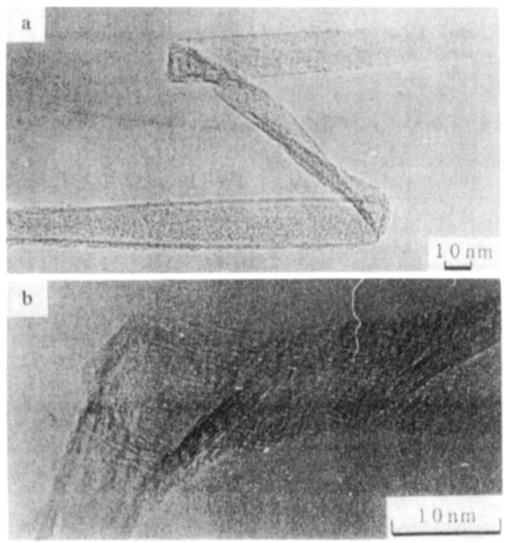
\includegraphics[width=0.55\columnwidth]{physicalcnt.png}
	\caption{ 	\label{CNT}
		Osservazione diretta dei CNTs che compiono delle torsioni (a)- doppio piegamento con una rotazione nel mezzo e (b)- una rotazionee completa. 
	}
\end{figure}
Osservazioni dirette, per lo più utilizzando TEM ad alta risoluzione, hanno dimostrato che i nanotubi di carbonio di piccolo diametro sono notevolmente flessibili. Come mostrato in Fig.\ref{CNT}, anche nanotubi di carbonio di diametro relativamente grande $(~ 10 nm)$ possono piegarsi e ruotare senza rompersi. È interessante notare che quando sono piegati o attorcigliati, i nanotubi sembrano appiattirsi nella sezione trasversale, in particolare accade ai nanotubi a parete singola con diametri superiori a 2,5 nm.\\
Gli studi teorici si sono concentrati su diversi aspetti, tra cui l'effetto della curvatura, del diametro del tubulo e della chiralità della struttura elettronica e il calcolo delle modalità di flessione per i tubuli.
Si è scoperto che i tubuli si ammorbidiscono in maniera inversamente proporzionale con il raggio, e si trova che la rigidità dei tubuli dipende dall'angolo chirale, infatti i tubuli a zigzag riscontrano una rigidità inferiore rispetto ai tubuli armchair.
I calcoli effettuati inerenti ai modi vibrazionali sono stati effettuati su lunghi CNT con alla base delle capsule semisferiche di $C_{60}$ e dunque con 30 atomi di carbonio infondo al tubulo, e sul corpo del tubulo costituiti da 100, 200 e 400 atomi di carbonio. Tali calcoli mostrano che la frequenza del modo di flessione diminuisce all'aumentare della lunghezza del tubulo. La rigidità di un fascio di questi tubuli si trova a superare quella dei materiali attualmente disponibili, offrendo eccezionali proprità meccaniche.\\
Le proprietà di superconduttività dei tubuli sono di grande interesse, essendo degli aggregati ad una dimensione. Tuttavia, finora non sono stati pubblicati resoconti di superconduttività nei tubuli di carbonio. Teorie si incentrano sulla possibilità che i singoli tubuli o i fasci paralleli di nanotubi possano mostrare tale comportamento. Ad esempio, nel caso di tubuli  multistrato, il problema sta nel fatto che la piccola distanza interplanare tra questi tubuli cilindrici (\SI{3.4}{\angstrom}), impedisce l'introduzione degli elementi tra gli strati di tubuli. Una possibilità per l'osservazione futura della superconduttività nei tubuli potrebbe comportare l'introduzione di un drogante a trasferimento di carica o di un metallo superconduttore nello spazio interstiziale tra tubuli in una matrice, o nel nucleo cavo del tubulo cilindrico . È già stato dimostrato che l'azione capillare può causare l'introduzione di specie ospiti nel nucleo cavo di un nanotubo di carbonio.

\subsection{Applicazioni dei nanotubi di carbonio}
I CNT possiedono molte proprietà uniche insieme alle proprietà fisiche di cui sopra. I dati statistici indicano chiaramente che dagli anni 2012-2013 la produzione commerciale di CNT ha superato diverse migliaia di tonnellate l'anno a causa delle sue vaste applicazioni nello stoccaggio di energia, parti automobilistiche, scafi per imbarcazioni, articoli sportivi, filtri per l'acqua, elettronica sottile, rivestimenti, attuatori e schermi elettromagnetici. Attualmente i CNT sono principalmente utilizzati per i materiali compositi strutturali, i display a pannello piatto (FPD), lo stoccaggio di gas ed energia, il rivestimento tecnico assorbente per radar e microelettronica, gli ultra-condensatori, punte di microscopi a forza atomica (AFM), batterie con maggiore durata, biosensori e così via.
I CNT sono strati di carbonio dello spessore di uno o due atomi e hanno una flessibilità molto elevata, quindi i nanotubi potrebbero essere utilizzati negli strumenti di scansione.  L'inconveniente principale dei CNT è la vibrazione dei nanotubi dovuta alla notevole lunghezza ed elasticità; tuttavia, questo problema potrebbe essere risolto in futuro da strumenti di controllo della crescita in lunghezza dei CNT che sono in fase di realizzazione.
I CNT hanno molte caratteristiche distintive che possono essere impiegate per assemblare sensori di nuova generazione e sono già stati sviluppati sensori basati su CNT di altissima qualità. Anche per questo si ritiene che gli SWCNT possano essere impiegati come attuatori elettromeccanici, simulando il meccanismo dell'attuatore presente nei muscoli naturali. Gli SWCNT dunque possono essere usati come sensori chimici miniaturizzati. 
Il transistor "ad effetto di campo" è un importante dispositivo a tre terminali costituito da un solo SWNT semiconduttore. Quando viene applicata una tensione, i nanotubi si convertono da uno stato di conduzione a uno stato di non conduzione. I transistor CNT possono essere poi uniti e, di conseguenza, funzionano come un interruttore logico, componente base dei computer. \\
Franklin et al. fabbricarono un transistor di nuova generazione costituito da un canale di 9 nm costituito da SWCNT. Quando viene applicata una tensione all'elettrodo, la corrente elettrica passa dall'elettrodo di source all'elettrodo di drain. Uno strato spesso 3 nm di ossido di afnio fornisce sufficiente interazione elettrostatica tra l'attacco e gli SWCNT. \\
I supercondensatori (SC, noti anche come ultracondensatori) sono dispositivi elettrochimici ad alta capacità. Questa caratteristica unica li rende utili per dispositivi che richiedono una piccola quantità di corrente e bassa tensione. A volte, i supercondensatori svolgono la funzione di una batteria elettrochimica a bassa tensione ricaricabile che ha una capacità molto elevata ed è adatta per i vari dispositivi elettronici. 

\chapter{Nanoschiuma di carbonio}
\textit{Interamente ripreso da Frese et al. \cite{foamm}.} \\
Le nanoschiume sono di notevole interesse per la loro struttura unica, che si trova tra due e tre dimensioni, consentendo la realizzazione molti nuovi tipi di materiali con funzioni promettenti per le tecnologie future. 
Le principali domande a cui ancora si deve rispondere sono relative ai metodi di sintetizzazione per la formazione, alla morfologia della schiuma e alle proprietà elettroniche e vibrazionali.
\section{Sintetizzazione e struttura del reticolo}
La nanoschiuma di carbonio si produce in diversi modi:\\
\begin{itemize}
	\item Tramite ablazione laser pulsata del carbonio vetroso in atmosfera di argon o della grafite in azoto liquido;
	\item La deposizione a laser pulsato, che è stata inoltre utilizzata per la fabbricazione di elettrodi di nanoschiuma di carbonio.
	\item La  carbonizzazione idrotermale a bassa temperatura del saccarosio. Tramite tale metono si è in grado di formare nanoschiuma di carbonio di alta qualità, infatti le schiume tendono ad essere composte da sfere micrometriche di carbonio prevalentemente $sp^2$ che formano una intelaiatura tridimensionale. Queste cosiddette microperle vengono solitamente rilevate come singole unità, che sono debolmente connesse, formando la struttura di schiuma.\\
\end{itemize}

\begin{figure}[h!] 
	\centering \label{foam}
	\includegraphics[width=0.55\columnwidth]{nanofoam.png}
	\caption{ 	
		Immagini al microscopio a ioni elio (HIM) di nanoschiuma di carbonio a bassa densità (a, b) e ad alta densità (c, d), con diversi ingrandimenti.}
\end{figure}
Le microperle hanno dimensioni ridotte. La morfologia del campione è abbastanza uniforme su ampie aree. Occasionalmente, le microperle crescono insieme formando unità più grandi, tuttavia, nella maggior parte dei casi, le microperle sono separate l'una dall'altra. In Fig. \ref{foam} (c), (d), ritroviamo della schiuma ad alta densità. Qui, le singole sfere di carbonio sono di dimensioni maggiori e mostrano una forte tendenza alla coesione.  
\section{Proprietà fisiche e utilizzi}
I materiali in nanoschiuma presentano proprietà fisiche derivanti da una miscela di atomi di carbonio con ibridazione $sp^2$ e $sp^3$. La struttura delle microperle si basa su una rete tridimensionale di tipo $sp^2$, la cui morfologia deriva dalla curvatura e dall'interconnessione dei piani basali grafitici.\\
Prendiamo in esame un tipo di nanoschiuma di carbonio che abbia una bassa densità e la struttura di una rete di grafene interconnessa.\\
A seconda delle condizioni di formazione, gli atomi di carbonio $sp^2$ possono o meno dar luogo ad anelli pentagonali ed eptagonali con interconnessioni di tipo $sp^3$ incorporate nella rete esagonale. I risultati mostrano che la combinazione di vari tipi di anelli e strutture ibride $sp^2-sp^3$ Può generare una una vasta varietà di strutture geometriche (e quindi di nanoschiume).\\
A causa della presenza di elettroni spaiati, dovuti a difetti nella struttura, la nanoschiuma mostra proprietà paramagnetiche e al di sotto di $-183 ^\circ C$ (punto di Curie) diviene ferromagnetica. \\

Tra i possibili usi sie ne evidenziano due: per l'immagazzinamento dell'idrogeno da sfruttare poi in pile a combustibile e l'uso vario in campo medico per aumentare la risoluzione delle immagini catturate dalla risonanza magnetica, ma anche nel trattamento anticancro, producendo una localizzazione del calore nella sede del tumore. \\
Vi sono poi dei sottoprodotti diversi della nanoschiuma di carbonio: la schiuma di nanotubi di carbonio è considerata utile nel trattamento delle acque e nella pulizia delle fuoriuscite di petrolio. La carta di nanoschiuma di carbonio viene proposta per applicazioni di stoccaggio dell'energia. I composti di nanoschiuma di carbonio possono essere utilizzati per elettrodi di condensatori elettrochimici con potenziale applicazione in supercondensatori elettrochimici ad alta densità di energia.
\chapter {Carbonio amorfo}
Il carbonio amorfo non presenta struttura cristallina.\\ 
Rientrano dunque in questa categoria tutti i prodotti della sintetizzazione di strutture amorfe, incluse le forme chiamate carbon black, activated carbon, charcoal, coal, e coke anche se all'esaminazione a raggi X risultano avere un grado molto basso di ordine locale (come se avessero dei piccoli agglomerati ordinati).
\section{Sintetizzazione e scoperta}
Fu scoperto nel 2011, ottenuto in laboratorio da Yu Lin et al. \cite{lin} comprimendo il carbone vetroso (una combinazione di vetro e grafite) a più di 400.000 volte la normale pressione atmosferica. \\
A causa delle loro numerose applicazioni industriali, i materiali costituiti da carbonio non cristallino hanno ricevuto recentemente molta attenzione. Questa classe di materiali può essere prodotta a basso costo mediante deposizione chimica da vapore (CVD) e da depositazione su superfici sottoforma di film sottili e duri, che presentano una buona biocompatibilità e inerzia chimica.\\
In questi film, la quantità di carbonio in forma $sp^3$, $sp^2$ e $sp$, insieme alla presenza o assenza di idrogeno, influenza la rigidità del rivestimento.\\
Il carbonio amorfo tetraedrico (ta-C) si sintetizza attraverso la tecnica “filtered cathodic vacuum arc” in cui si vaporizza in materiale che si trova su di un bersaglio catodico. Il materiale vaporizzato si condensa su un supporto formando un film sottile.\\
Il carbonio amorfo polimerico (PLC) e i film di carbonio idrogenati sono stati sitetizzati invece mediante deposizione chimica da vapore potenziata al plasma.
\section{Reticolo Cristallino}
Il carbonio amorfo (a-C) è una rete altamente disordinata di atomi di carbonio che hanno prevalentemente legami di tipo $sp^2$, con circa il $10\%$ di legami $sp^3$  e rari legami di tipo $sp$. Sebbene il carbonio amorfo non abbia un ordine a lungo raggio (regolarità nella disposizione atomica), è presente un ordine a corto raggio (disposizione regolare e prevedibile degli atomi su una breve distanza, che non persiste a lunga distanza). Poiché la natura dell'ordine a corto raggio varia significativamente da un metodo di sintetizzazione a un altro, anche le proprietà del film di carbonio amorfo variano a seconda dei metodi di preparazione.\\
I due parametri più significativi per la caratterizzazione dell'ordine a corto raggio sono il rapporto tra i legami $sp^2/sp^3$ e il contenuto di idrogeno. Gli atomi di carbonio con legame $sp^2$ possono raggrupparsi in minuscole regioni stratificandosi e deformandosi, mentre gli $sp^3$ possono sia raggrupparsi che separarsi, come pure le impurità di idrogeno, che molto spesso sono presenti e hanno il ruolo di riempire i legami liberi (Fig. \ref{yaas}).
\begin{figure}[h!]
	\centering
	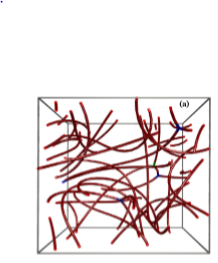
\includegraphics[width=.35\textwidth]{Amorph.png}\hfil
	\includegraphics[width=.3\textwidth]{Amorph1.png}\hfil
	\includegraphics[width=.35\textwidth]{Amorph2.png}
	
	\caption{È stata utilizzata la seguente combinazione di colori: gli atomi di $sp^3$ sono mostrati in verde, $sp^2$ in blu e sp in rosso. (a) Una rete di carbonio amorfo  ricca di $sp$. (b) Una struttura mista $sp^2 / sp^3$, in cui le due fasi sono distinte. (c) Un'altra struttura mista $sp^2 / sp^3$ in cui non ci sono fasi visibilmente distinte in questo caso.}\label{yaas}
\end{figure}
In genere il carbonio amorfo è anche formato da neutroni, elettroni, o da materiali a base di carbonio irradiati da fasci ionici, che precedentemente avevano un ordine strutturale maggiore.\\

Non si tratterà la dispersione fononica per via della mancanza di studi eseguiti a riguardo, avendo il carbonio amorfo un alto grado di disordine.
\section{Proprietà fisiche e applicazioni possibili}
\subsection{Proprietà fisiche}
Un foglio di grafene $sp^2$ è un semiconduttore a gap zero. L'introduzione di un certo grado di disordine e di impurità in una struttura del genere crea un semiconduttore con dei stati localizzati vicino al livello di Fermi e un intervallo di banda efficace tra bande piene e bande di conduzione vuote. Maggiore è il disordine, maggiore è la concentrazione dei legami $sp^3$, e maggiore è il gap. \\
Il carbonio amorfo sintetizzato tramite processo di deposizione chimica da vapore tende ad avere una conducibilità elettrica a temperatura ambiente più alta $\sigma_{RT}=10^3 \Omega^{-1}cm^{-1}$ ed un più basso gap ($E_g \sim0.4-0.7 eV$) rispetto  ad un a-C prodotto attraverso la sintetizzazione di tipo "Filtered cathodic vacuum arc" per il quale si ottengono $\sigma_{RT}=10^2 \Omega^{-1}cm^{-1}$ e $E_g \sim 0.4- 3.0eV$.
Poiché il carbonio amorfo non ha un ordine a lungo raggio, è consuetudine caratterizzare i campioni a-C in termini delle loro funzioni di distribuzione radiale misurate in un esperimento di diffrazione (elettronica, raggi X o neutronica). I campioni di carbonio amorfo sono anche caratterizzati in termini di densità rispetto alla grafite ($\rho= 2,26 g / cm^3$) per specificare la densità di “aggrovigliamento” del film. Il rapporto tra il legame $sp^2 / sp^3$ nei campioni a-C è solitamente determinato grazie alla spettroscopia, ad esempio mediante risonanza magnetica nucleare (NMR), o con spettroscopia di elettroni a perdita di energia.\\
Successivamente, con la scoperta di nuove forme di a-C, è stata evidenziata l'influenza di alcune caratteristiche rispetto ad altre in base a come è stato sintetizzato il carbonio amorfo. La complessità intrinseca dei vari tipi di a-C ()determinata dalla evetuale presenza di anelli, dalla proporzione di legami ibridi $sp$, $sp^2$ e $sp^3$ e la dimensione degli agglomerati) può spiegare la difficoltà nell'ottenere una legge che leghi la densità ed il modulo di copressione alle coordinate spaziali che descriva in maniera universale tutte le tipologie di a-C.
\subsection{utilizzi}
Ciascuna delle forme amorfe di carbonio ha il suo carattere specifico e, quindi, ciascuna ha le sue particolari applicazioni. Tutti sono prodotti di ossidazione e altre forme di decomposizione di composti organici. Il coal ed il coke, ad esempio, sono ampiamente utilizzati come combustibili. Il crachoal è usato come agente assorbente, filtrante e come combustibile; utempo addietro era ampiamente usato come ingrediente nella polvere da sparo. (I coals sono carbonio puro mescolato a quantità variabili di composti del carbonio). \\
Oltre al suo utilizzo nella produzione di inchiostri e vernici, il carbon black viene utilizzato come additivo nella gomma dei pneumatici e nelle plastiche, per migliorare le sue qualità nell'usura; è usato poi come colorante in inchiostri e riducente in metallurgia. \\
L'activetad carbon, che presenta un’elevata area superficiale, è utilizzato per purificare gas e liquidi, in medicina e nell’alimentazione. \\
Grazie alle loro proprietà ottiche, il carbonio amorfo si utilizza a partire dal 2011 come rivestimento antiriflesso per celle solari in silicio cristallino.
\chapter{T-Carbon (2011)}

\textit{Interamente ripreso da Sheng et al. \cite{TCAR}.}\\

Questa struttura fu solo teorizzata nel 2011, e sintetizzata poco più avanti. Può essere ottenuta sostituendo ciascun atomo nel reticolo del diamante con un tetraedro di atomi di carbonio, formando un reticolo cristallino cubico che possiede lo stesso gruppo spaziale del diamante. Questa solido molecolare è quindi soprannominato T-carbon (da tetraedrico).

\section{Reticolo Cristallino}

L'idea è ispirata dalla creazione del tetraedrano, derivato dal metano dalla sostituzione di ogni atomo di carbonio nel metano con un tetraedro di carbonio.\\
Allo stesso modo possiamo costruire un nuovo allotropo del carbonio sostituendo ogni atomo di carbonio nel diamante con un tetraedro di carbonio , come indicato in Fig.\ref{TCarb}.\\
\begin{figure}[h!] 
	\centering \label{TCarb}
	\includegraphics[width=0.55\columnwidth]{TCarbon.png}
	\caption{ 	Rappresentazione schematica della struttura del T-Carbon. (a) La struttura cristallina cubica che si ottiene sostituendo ciascun atomo in diamante con un tetraedro di carbonio, dove la costante del reticolo è \SI{7,52}{\angstrom} . le immagini (b), (c), (d) Viste da [100], [110] e [111] direzioni di T-carbon, rispettivamente.	}
\end{figure}
Fortunatamente, la stabilità di una tale struttura è stata verificata e ottimizzata. In questa nuova struttura, ogni cella unitaria contiene due tetraedri con otto atomi di carbonio, e la costante del reticolo è di circa L=\SI{7,52}{\angstrom}. I tre vettori unitari sono a =(L/2)(1,1,0), b =(L/2)(0,1,1) e c=(L/2)(1,0,1).\\
Esistono due distinti legami con lunghezza  \SI{1.502}{\angstrom} e \SI{1.417}{\angstrom} entrambi legami intertetraedro per il T-carbon. Entrambi sono più piccoli di quelli del diamante. Ci sono anche due diversi angoli di legame, $60^\circ$ nel tetraedro e $144.74^\circ$ tra due legami non equivalenti. Il primo è molto inferiore a quello del diamante (di $109,5^\circ$) il che probabilmente porta all'aumento dell'energia totale.

\section{Proprietà fisiche e applicazioni possibili}
Il T-carbon è cineticamente stabile e con una densità di $1,50 \: g / cm^3$. Le strutture elettroniche rivelano che si tratta di un semiconduttore con un band gap diretto attorno a 3,0 eV.\\ La caratteristica notevole è che la densità all'equilibrio ($\rho$) del T-Carbon è la più piccola ($1:50 g/cm^3$). Il suo modulo di compressibilità è solo il 36,4\% del diamante cubico; è infatti possibile immagazzinare molecole di idrogeno nel T-carbon.\\
Presentano una densità e un modulo di compressibilità  molto più bassi rispetto al diamante e tutte queste caratteristiche sopra elencate suggeriscono che il T-carbon, una volta sintetizzato, potrebbe avere ampie applicazioni.
Dopo la sintetizzazione, il T-carbon può avere ampie applicazioni nella fotocatalisi, nell'assorbimento, nell'immagazzinazione dell'idrogeno e nella costruzione di materiali aerospaziali.\\



\chapter{Q-Carbon (2015)}
\textit{Interamente ripreso da Narayan et al. \cite{QCAR}.}
\section{Sintetizzazione e reticolo cristallino}
Il Q-carbon si forma come risultato della tempra del carbonio liquido sottoposto ad una super-sopraffusione alla pressione atmosferica. Esso svolge un ruolo critico nella formazione del diamante. È stato ipotizzato che il carbonio liquido possa esistere all'interno dei nuclei dei pianeti di Urano e Nettuno, come una fase termodinamicamente stabile ad alte pressioni e temperature, e contribuire al compo magnetico di tali pianeti. Tale scoperta può anche dunque  spiegare il ferromagnetismo nel nostro sistema planetario e nelle forme termodinamicamente stabili di carbonio, grafite, diamante, carbonio liquido e vapore. \\
Il Q-Carbon può essere ottenuto mediante un processo di fusione del  carbonio amorfo causata da laser che emettono impulsi ottici con durata del nanosecondo, in cui lo stato di sopraffusione è di circa 4000 K, ossia circa 1000 K sotto il punto di fusione della grafite. \\
La retta tratteggiata a 4000K nel diagramma di fase \ref{phases}, che connette il punto triplo di grafite, carbonio liquido e diamante a 5000K rappresenta questo stato di super-sopraffusione, che a seguito della tempra sfocia nella formazione di Q-Carbon ad una temperatura leggermente inferiore a 4000K. Da tale allotropo del carbonio poi siamo in grado di creare nanodiamanti, microdiamanti e film sottili. \\
\begin{figure}[h!] 
	\centering \label{Qcarbont}
	\includegraphics[width=0.55\columnwidth]{Qcarboon.png}
	\caption{ 	Formazione del Q-carbon, nanodiamanti e microdiamanti dopo un impulso laser: (a) Micrografia SEM che mostra il Q-carbon dopo singolo impulso laser del laser ArF (lunghezza d'onda 193nm, durata dell'impulso 20ns) a 0,5 $J/cm^2$ o regioni esterne di $0,6 J/cm^2$ ; (b) formazione di microdiamanti dalle pieghe verso il bordo del campione di 0,6 $J/cm^2$; (c) nano- e microdiamanti nel mezzo del campione di 0,6 $J/cm^2$; e (d) solo microdiamanti che coprono l'intera area in alcune regioni di 0,6 $J/cm^2$ di campione.
		}
\end{figure}
Lo strato di carbonio in processo di sopraffusione si forma vicino alla superficie del film, che può rompersi in una struttura rassomigliante alle strutture cellulari (la struttura filamentare il figura \ref{Qcarbont}) in seguito al processo di tempra che porta alla formazione di un nuovo stato di carbonio.
La formazione di una struttura cellulare deriva dall'instabilità di una superficie solida a contatto con del liquido. La figura mostra una struttura cellulare (micrografia SEM) di filamenti di Q-carbon (200-500 nm) formati grazie all'irradiazione laser con impulso $0,5 J \cdot cm^{-2}$ del laser ArF. Il Q-Carbon risultante da tale processo ha una matrice di carbonio amorfo principalmente con legami $sp^3 (> 75\%)$ in cui sono incorporati nanocristalli di diamante come mostrato in figura. \\
Il resto dei legami sono $sp^2$: lo spettro Raman del Q-Carbon mostra una frazione molto grande di carbonio legato $sp^3$ (75\% -85\%), insieme al picco del diamante a $1333 cm^{-1}$ e picchi con legame $sp^2$ a $1140 cm^{-1}$ e $1580 cm^{-1}$.
La cosa più interessante di tutte è che il Q-carbon manifesta proprietà ferromagnetiche a temperatura ambiente e al di sopra di essa.
\section{Proprietà fisiche e applicazioni possibili}
Si prevede che il  Q-Carbon possegga nuove proprietà fisiche, chimiche, meccaniche e catalitiche, infatti vi è una notevole riduzione di volume quando il carbonio amorfo viene convertito in Q-carbon.\\
Il Q-carbon presenta una buona conducibilità elettrica, essendo di natura un semiconduttore metallico. Presenta una maggiore emissione di campo e una durezza molto elevata. \\
Presenta anche nuove proprietà, tra cui il ferromagnetismo a temperatura ambiente (RTFM) e una maggiore durezza e emissione di campo. Va sottolineato che la presenza di una concentrazione di $sp^3$ simile al film di carbonio amorfo depositato non risulta in RTFM. \\
Dal Q-Carbon si ricavano ed elaborano nanodotti, microcristalli, nanoaghi, microaghi e film sottili monocristallini di diamante piuttosto economici su substrati pratici e termosensibili per una varietà di applicazioni che vanno dalle polveri abrasive, nuove proprietà catalitiche, display intelligenti e miriadi di applicazioni biomediche e microelettroniche e nanoelettroniche con un impatto massimo sull'uomo. 
\chapter{Novamene (2017)}
\textit{Interamente ripreso da Burchfielda et al.\cite{NOVA}}\\

Tutta una nuova classe di allotropi.\\

La base di questa nuova classificazione risiede nel concetto di combinazione fra il diamante esagonale (con legami $sp^3$ - lonsdaleite) e il carbonio che si dispone ad anello attorno ad esso (carbonio con leami $sp^2$ - grafene). Poiché la lonsdaleite funge da isolante e gli anelli fungono da conduttori, questi materiali hanno potenziali applicazioni per transistor e altri componenti elettronici.


\section{Reticolo Cristallino}
La disposizione  degli anelli esagonali uno adiacente all'altro è detta fusenes e sono le strutture rappresentate in fig. \ref{nononova}. \\
\begin{figure}[h!] 
	\centering \label{nononova}
	\includegraphics[width=0.55\columnwidth]{Nova.png}
	\caption{ 	Uno schizzo di tutte le possibili combinazioni non equivalenti di anelli esagonali in un piano, collegando fino a quattro esagoni.
	}
\end{figure}
Questa immagine fornisce una "lista" di vari tipi di configurazioni $sp^2$ dei composti di novamene. Affronteremo il primo tipo, essendo tutti gli altri una conseguenza di questo. \\
\begin{figure}[h!] 
	\centering \label{novacarbon}
	\includegraphics[width=0.86\columnwidth]{SimpleNovamene.png}
	\caption{ 	La struttura del cristallo novamene single-ring; (a): vista dall'alto; (b): vista laterale. Gli atomi di entrambe le figure sono contressegnati dagli stessi colori. La maggior parte degli atomi è legata a quattro altri atomi, ad eccezione di quelli ciano negli anelli esagonali A che sono $sp^2$ e legati ad altri tre atomi. Linea tratteggiata: il limite della cella unità periodica.}
\end{figure}
La più semplice unità di grafene è quella composta da un solo anello a sei atomi di carbonio. Quando questo anello è circondato dalla lonsdaleite (con legame $sp^3$), essa si dispone in 3 anelli costituiti da cinque atomi di carbonio e 3 anelli costituiti da sette atomi di carbonio, che si assemblano insieme come illustrato in Fig. \ref{novacarbon}. \\
Una delle caratteristiche chiave di questo allotropo del carbonio è che la più semplice struttura unitaria può essere periodicamente riprodotta per costruire una struttura 3D estesa. Il motivo che si crea è simile al modello di ripetizione fondamentale nelle "bucky-balls"; la differenza è che nel novamene la struttura dei 3 pentagoni che circondano un anello esagonale centrale rimane su di un piano, grazie agli anelli di carbonio a 7 atomi che spuntano dal piano A al piano B vicino. La distanza interplanare A-B calcolata è di \SI{2,5}{\angstrom}.\\

Sulla base dell'analisi eseguita qui sopra, è intuitivamente ovvio che esistono altri tipi di novamene, aumentando il numero di anelli esagonali racchiusi nella lonsdaleite. Ciò modifica il bilanciamento di $sp^2/sp^3$ in favore di $sp^2$, portando ad altre strutture, mostrati nelle Fig. \ref{twonovah}.
\begin{figure}[h!] 
	\centering \label{twonovah}
	\includegraphics[width=0.55\columnwidth]{twonovamene.png}
	\caption{  Modello "Ball-and-stick" del novamene a due anelli esagonali. I legami viola corrisondono alle connessioni di tipo $sp^2$ mentre i legami bianchi agli $sp^3$.
	}
\end{figure}

\section{Proprietà fisiche e applicazioni possibili}
La varietà di strutture del novamene attualmente descritte (che combinano l'azione del core di grafene conduttore circondato dalla lonsdaleite isolante) può rivelarsi utile per diverse applicazioni. Ad esempio, nella produzione di circuiti integrati, l'incorporazione del novamene fornirebbe un'elevata mobilità dei portatori di carica, dovuta al nucleo centrale di grafene, insieme a rigide proprietà meccaniche. 
La densità degli stati è molto simile a quella della lonsdaleite fatta eccezione per le bande vicino all'energia di Fermi, che sono separate da una distanza piuttosto piccola. Ciò indica che la struttura del novamene è quella di un semiconduttore caratterizzato da un gap indiretto di 335 meV. \\
L'anisotropia della struttura del novamene risulta utile nelle applicazioni di raccolta dell'energia solare.

\section{Sintetizzazione e scoperta}
La lonsdaleite ha la capacità di "attaccarsi" al grafene per formare centinaia di allotropi del carbonio. Ciò potrebbe anche spiegare ineffetti la differenza in durezza fra i campioni di lonsdaleite riscontrata: vi potrebbe essere una percentuale sostanziale di difetti $sp^2$ che da luogo a strutture del tipo del novamene.\\
Inoltre, un'analisi strutturale dettagliata potrebbe dimostrare che il Q-Carbon è una disposizione disordinata contenente una percentuale sostanziale di novamene di primo tipo (single ring), o più frequentememnte novamene formato da anelli multipli. 
\chapter{Protomene (2018)}
\textit{Interamente ripreso da Delodovici et al. \cite{PROTO}.}\\

La struttura del protomene condivide alcuni concetti generali con quella del novamene precedentemente studiato, ma con significative novità. Nel protomene, 6 atomi su 24 (rispetto a 2 su 26 nel novamene) possono avere una geometria $sp^2$ perfettamente planare, dalla quale possono quindi uscire dal piano per creare legami relativamente deboli con gli atomi gemelli della successiva cella reticolare impilata verticalmente.\\
Secondo l'esempio del novamene, ci si aspetta che questa nuova formazione di legami diminuisca l'energia totale di circa 1 eV per legame e induca un cambiamento sostanziale nelle proprietà elettroniche.

\section{Reticolo Cristallino}
Come il novamene, la struttura del protomene ha tre assi di simmetria, che sono compatibili con la cristallizzazione in un reticolo esagonale. Si è costruito un classico modello “ball and stick” e lo si è adattato a un classico reticolo, con una simmetria di ripetizione, come riportato in Fig. \ref{protocarbon}. \\
\begin{figure}[h!] 
	\centering \label{protocarbon}
	\includegraphics[width=0.75\columnwidth]{Protomene.png}
	\caption{ Modello "ball-and-stick" del protomene, frontale e laterale.}
\end{figure}
Si è identificata la cella unitaria primitiva: contiene 24 atomi, ed è abbozzata da una linea tratteggiata in Fig. \ref{protocarbon}.\\
Nella figura si evidenziano gli atomi $sp^2$ in rosso: un gruppo di 4 atomi (etichettati 1, 3, 5 e 7) si trovano negli angoli della cella, più altri due (etichettati 9 e 11) isolati all'interno della cella. Gli atomi marcati con numero pari si ripropongo in posizioni equivalenti nello strato successivo (fig.\ref{protocarbon}-b). Tutti i 18 atomi rimanenti di colore grigio sono nativi di ibridazione $sp^3$.\\

Rispetto al novamene, la principale novità strutturale di questo nuovo allotropo consiste nell'assenza di anelli esagonali. Il protomene ha solo gruppi di al massimo quattro atomi $sp^2$ legati insieme. Questi atomi $sp^2$ hanno la possibilità di formare ulteriori legami con atomi simili in piani cristallini adiacenti.
\section{Proprietà fisiche e applicazioni possibili}
La densità degli stati risulta abbastanza liscia, nonostante la natura piuttosto piatta di alcune regioni delle bande. Il divario tra la banda di valenza e la banda di conduzione è l'unico divario in questa regione di energia, e la densità degli stati cambia da relativamente piccola vicino al divario stesso a qualche elettronvolt lontano da esso, sia nella valenza che nella regione di conduzione. \\

Il Protomene si qualifica come un nuovo semiconduttore potenzialmente utile. Il gap di banda di energia è molto vicino a quello del nitruro di gallio (GaN) che è di circa 3,4 eV a temperatura ambiente. Di conseguenza, il protomene possiede proprietà semiconduttive simili al GaN, che possono consentirgli di avere applicazioni per dispositivi elettronici ad alta potenza e / o ad alta frequenza. Potrebbe avere in realtà caratteristiche migliori, essendo che il protomene è un allotropo del carbonio, dunque ha un solo elemento e il controllo dei difetti potrebbe essere più facile rispetto a GaN.\\
Il protomene può trovare applicazioni in componenti opto-elettronici, ad esempio generando luce blu o UV può essere utilizzato come LED o come filtro UV in ottica. Inoltre, potrebbe avere anche maggiori applicazioni rispetto ai CNT nei dispositivi a semiconduttori. In effetti, un ostacolo da superare nella fabbricazione di CNT è controllare se il CNT è un semiconduttore metallico. Si prevede invece che il protomene sia semiconduttore fino a una temperatura di transizione.\\
È probabile che l'espansione termica del protomene giochi contro il legame interplanare. Pertanto, al diminuire della temperatura, è probabile che si verifichi una transizione di fase strutturale dalla struttura che troviamo in fig. \ref{protocarbon} a 24 atomi, ad una struttura a 48 atomi a semiconduzione. Di conseguenza, questa transizione di fase fornirebbe un filtro ottico sensibile alla temperatura, dato che, all'aumentare della temperatura, la banda proibita si chiude rapidamente, molto più velocemente che nel diamante e nel silicio. Inoltre, l'eventuale transizione alla fase metallica ad alta temperatura del protomene ha potenziali applicazioni di commutazione ottica ed elettrica a temperatura controllata. Inoltre, dato il crescente numero di legami $sp^2$, questa transizione di fase potrebbe compromettere la durezza del protomene nella fase di sintetizzazione. Pertanto, si prevede che il protomene presenti un abbassamento significativo della durezza al crescere della temperatura. \\

In futuro, Delodovici et al. prospettano di continuare la ricerca di nuovi allotropi di carbonio, ad esempio considerando la possibilità di interconnettere catene $sp$ con un impalcatura $sp^3$.


\chapter{D-Carbon (2018)}
\textit{Interamente ripreso da Fan et al. \cite{DCAR}.} \\

Il D-Carbon è un allotropo del carbonio con reticolo cristallino ortorombico $sp^3$ (gruppo spaziale $D_{2h}^5$ con 6 atomi per cella). I calcoli per trovare l'energia totale del sistema dimostrano che il D-carbon è energeticamente più favorevole rispetto a molte altre strutture proposte in precedenza. Ad esempio, questa nuova fase è dinamicamente, meccanicamente e termicamente più stabile della grafite da pressione zero fino a oltre 63,7 GPa.
\section{Reticolo cristallino}
\begin{figure}[h!] 
	\centering \label{DCarbon}
	\includegraphics[width=0.75\columnwidth]{DCarbon.png}
	\caption{ Struttura cristallina del D-Carbon: (a)- vista in prospettiva e rispettivamente (b),(c),(d) vista lungo gli assi \textbf{c}, \textbf{a}, e \textbf{b}.}
\end{figure}
La Figura \ref{DCarbon} mostra il modello strutturale ottimizzato del D-carbon. Questa struttura ha una cella unitaria primitiva ortorombica contenente sei atomi di C, in figura delimitata dalla linea blu. A pressione zero, i parametri di reticolo sono a =\SI{ 2.52}{\angstrom}, b =\SI{3.91}{\angstrom}, e c =\SI{3.81}{\angstrom}, con un gruppo spaziale altamente simmetrico. A pressione zero, la distanza fra due atomi di carbonio a riposo di C-C sono rispettivamente di \SI{1,60}{\angstrom} e \SI{1,54}{\angstrom}. Notiamo che il D-carbon non è solo più stabile di alcuni allotropi del carbonio teoricamente previsti, ma anche energeticamente più favorevole di diverse strutture del carbonio sperimentalmente realizzate (cioè il $C_{20}$ e T-carbon), il che implica che il D-carbon potrebbe essere sintetizzato. \\
Per valutare ulteriormente la stabilità di questo allotropo, abbiamo anche calcolato la sua energia coesiva $E_{coh} = [6E_C - E_ {total}]/6$, dove $E_{total}$ ed $E_C$ sono l'energia totale del D-carbon e di un singolo atomo di C, rispettivamente.
Essa risulta essere pari a $7.48 eV/atom$, apparentemente superiore al T-carbon precedentemente proposto ($6,573 eV / atom$). Ciò ci suggerisce che il D-carbon presenta un reticolo fortemente legato.

\section{Proprietà fisiche e utilizzi}
Con l'aumento della pressione, il D-carbon risulta più stabile della grafite fino a sopra i 63.7 GPa. La frequenza fononica più alta si trova nel punto con un valore di $\sim1333 cm^{-1}$, che è inferiore alla grafite ($\sim1600cm^{-1}$), ma vicino alla grafite a 63.7 GPa. \\
Il carbonio D è significativamente più morbido del diamante. Secondo la convenzione generalmente accettata, i materiali superduri hanno un $H_\nu$ superiore a 40 GPa, quindi, il carbonio D può essere considerato un materiale superduro.

\section{Sintetizzazione}
Il D-carbon si dovrebbe sintetizzare attraverso il processo di tempra generando una fase metastabile a pressione atmosferica e basse temperature. \\
Una corrispondenza soddisfacente del modello con il pattern ottenuto dalla diffrazione a raggi X simulato e misurato indica la possibile presenza di D-Carbon nella fuliggine o nella polvere da sparo. Data l'elevata stabilità dinamica del D-carbon e considerando il rapido sviluppo di tecniche sperimentali che hanno recentemente sintetizzato alcuni nuovi allotropi del carbonio, ci aspettiamo che il D-carbon possa essere fabbricato sperimentalmente a breve.

\begin{thebibliography}{99}
\bibitem{Qian}
Fancy Qian Wang, Ming Hu and Qian Wang, \textit{Ultrahigh thermal conductivity of carbon allotropes with correlations to the scaled Pugh ratio} Journal of Materials Chemistry \textbf{13 February 2019} 


\bibitem{melissinos}
Santosh K. Tiwari, Vijay Kumar, Andrzej Huczko, R. Oraon, A. De Adhikari, G. C. Nayak,
 \textit{Magical Allotropes of Carbon: Prospects and Application}, arcticle in \textit {Critical Reviews in Solid State and Material Sciences},  Vol. 41, No. 4 \textbf{ · November 2016 }

\bibitem{melissinos}
B Gopalakrishnan, S V Subramanyam,  \textit{Many Phases of Carbon }, Resonance \textbf {· December 2002}

\bibitem{melissinos}
M. S. Dresselhaus, G. Dresselhaus, P. C. Eklund,  \textit{Science of Fullerenes and Carbon Nanotubes }, Academic Press, University of Kentucky
\textbf {· 1995}


\bibitem{melissinos}
  Jagdish Narayan, and Anagh Bhaumik, \textit{Novel phase of carbon, ferromagnetism, and conversion into diamond }, Journal of Applied Physics 118, 215303
\textbf {· 2015}

\bibitem{melissinos}
Jagdish Narayan, and Anagh Bhaumik, \textit{Research Update: Direct conversion of amorphous carbon into diamond at ambient pressures and temperatures in air },  APL Material 3, 100702
\textbf {· 2015}
 

\bibitem{Kotr}
Sergiy Kotrechko, Igor Mikhailovskij, Tatjana Mazilova, Evgenij Sadanov, Andrei Timoshevskii, Nataliya Stetsenko and Yurij Matviychuk, \textit{Mechanical properties of carbyne: experiment and simulations},  Nanoscale Research Letters
\textbf {31 January 2015}

\bibitem{phono}
Alberto Milani, Matteo Tommasini, e Giuseppe Zerbi
\textit{Carbynes phonons: A tight binding force field}, The journal of chermical physics, 128, 064501 \textbf {2008}

\bibitem{melissinos}
Yu. P. Kudryavtsev, R. B. Heimann, S. E. Evsyuvov, \textit{Carbynes: advances in the field of linear carbon chain compounds},  JOURNAL OF MATERIALS SCIENCE 31 5557-5571
\textbf {1996}

\bibitem{melissinos}
Harry Marsh, Francisco Rodríguez-Reinoso, \textit{Activated Carbon},  Elsevier Ltd. \textbf {2006}

\bibitem{Mault}
J. Maultzsch, S. Reich, C. Thomsen, H. Requardt, e P. Ordejòn, \textit{Phonon Dispersion in Graphite},  PHYSICAL REVIEW LETTERS, Vol. 92, number 7 \textbf {20 February 2004}

\bibitem{melissinos}
Prithu Mukhopadhyay e Rakesh K. Gupta, \textit{Graphite, Graphene and their polymer nanocomposites}, CRC Press Taylor $\&$ Francis Group  \textbf {2013}

\bibitem{melissinos}
Hugh 0. Pierson, \textit{HANDBOOK OF CARBON, GRAPHITE, DIAMOND AND FULLERENES, Properties, Processing and Applications}, Noyes publications, Parck Ridge, New Jersey, U.S.A  \textbf {1993}

\bibitem{melissinos}
Wanda Andreoni, \textit{The Physics of fullerene-based and fullerene-related materials}, Physics and Chemistry of Materials with Low-Dimensional Structures, Vol.23  Springer Science+Business Media Dordrecht,  \textbf {2000}

\bibitem{melissinos}
L. Pintschovius, B. Renker, F. Gompf, R. Heid, S. L. Chaplot, M. Haluska, and H. Kuzmany, \textit{Inelastic Neutron Scattering Study of the External Vibrations in Single Crystal C60}, Physical review letters Vol.69, No.18 -  \textbf {November 1993}

\bibitem{melissinos}
R. R. Nair, P. Blake, A. N. Grigorenko, K. S. Novoselov, T. J. Booth, T. Stauber, N. M. R. Peres, A. K. Geim \textit{Fine Structure Constant Defines Visual Transparency of Graphene},  Science Express   \textbf {3 April 2010}

\bibitem{Saito}
R. Saito, G. Dresselhaus, and M. Dresselhaus, \textit{Physical Properties of Carbon Nanotubes.},  London: Imperial College Press, \textbf {1998}
 
\bibitem{Gray}
Dodd Gray, Adam McCaughan, Bhaskar Mookerji, \textit{Phonon Spectra of Graphene},  6.730—Physics for Solid State Applications \textbf {17 April 2009}

\bibitem{melissinos}
L. A. Falkovsky, \textit{Phonon Dispersion in Graphene},  Journal of Experimental and Theoretical Physics, Vol. 105, No. 2, \textbf {19 february 2007}

\bibitem{melissinos}
H.Tetlowa, J.Posthuma de Boerb, I.J.Forde, D.D.Vvedenskyb, J.Corauxcd, L.Kantorovich, \textit{Growth of epitaxial graphene: Theory and experiment},  Physics reports, Vol. 542,
 \textbf {20 September 2014}
 
 \bibitem{melissinos}
SashaStankovich, Dmitriy A.Dikin, Richard D.Piner, Kevin A.Kohlhaas, Alfred Kleinhammes, Yuanyuan Jia, Yue Wu, Son Bin, T.Nguyen Rodney, S.Ruoffa \textit{Synthesis of graphene-based nanosheets via chemical reduction of exfoliated graphite oxide}, Carbon, Vol. 45, \textbf {June 2007}

\bibitem{melissinos}
Mohammad Choucair, Pall Thordarson and John A. Stride, \textit{Gram-scale production of graphene based on solvothermal synthesis and sonication}, Nature Nanotechnology ·  \textbf {February 2009}

\bibitem{melissinos}
Minzhen Cai,Daniel Thorpe, Douglas H. Adamson and Hannes C. Schniepp, \textit{Methods of graphite exfoliation},Journal of Materials Chemistry,  \textbf { 22 August 2012}

\bibitem{Rustam}
Rustam Z. Khaliullin, Hagai Eshet, Thomas D. Kühne, Jörg Behler and Michele Parrinello, \textit{Nucleation mechanism for the direct graphite-to-diamond phase transition}, Nature materials,  \textbf { July 2011}

\bibitem{XIE}
Hongxian Xie, Fuxing Yin, Tao Yu, Jian-Tao Wang and Chunyong Liang, \textit{Mechanism for direct graphite-to-diamond phase transition}, Scientific reports, \textbf { July 2014}

\bibitem{dimondi}
V. S. Gorelika and N. S. Vasil’ev, \textit{Dispersion of Optical and Acoustic Phonons in Diamond and Germanium Crystals}, Inorganic Materials, Vol. 48, No. 5, pp. 462–468, \textbf {2012}

\bibitem{Kulni}
Boris Kulnitskiy, Igor Perezhogin, Gennady Dubitskya and Vladimir Blanka, \textit{Polytypes and twins in the diamond–lonsdaleite system formed by high-pressure and high-temperature treatment of graphite}, Structural Science, Crystal Engineering and Materials, \textbf { 30 July 2013}

\bibitem{qing}
Li Qingkun, Sun Yi, Li Zhiyuanc and Zhou Yu, \textit{Lonsdaleite – A material stronger and stiffer than diamond}, Science Direct, scripta materialia 65, \textbf{2011}

\bibitem{melissinos}
X. Ma, L. Shi, X. Hi, L. Li, G. Cao, C. Hou, Jiacheng, Li Chang, Lin Yang, Y. Zhong, \textit{Graphitization resistance determines super hardness of lonsdaleite,nanotwinned and nanopolycrystalline diamond}, Carbon 133 69-76, \textbf{2018}

\bibitem{melissinos}
F. H. Jornada, V. Gava, A. L. Martinotto, L. A. Cassol and C. A. Perottoni, \textit{Modeling of amorphous carbon structures with arbitrary structural constraints}, J. Phys.: Condens. Matter n. 22 395402 \textbf{2010}

\bibitem{lin}
Yu Lin, Li Zhang, Ho-kwang Mao, Paul Chow, Yuming Xiao, Maria Baldini, Jinfu Shu, and Wendy L. Mao,
\textit{Amorphous Diamond: A High-Pressure Superhard Carbon Allotrope} PHYSICAL REVIEW LETTERS, PRL 107, 175504,  \textbf{19 October 2011}

\bibitem{melissinos}
D. S. da Silva, A. D. S. Côrtes, M. H. Oliveira Jr., E. F. Motta, G. A. Viana, P. R. Mei, and F. C. Marques,
\textit{Application of amorphous carbon based materials as antireflective coatings on crystalline silicon solar cells} Journal of Applied Physics, 110, 043510  \textbf{2011}

\bibitem{foamm}
Natalie Frese, Shelby Taylor Mitchell, Christof Neumann, Amanda Bowers, Armin Gölzhäuser and Klaus Sattler,
\textit{A Fundamental properties of high-quality carbon nanofoam: from low to high density } Beilstein Journal Nanotechnology 7, 2065–2073  \textbf{2016}

\bibitem{QCAR}
Jagdish Narayan and Anagh Bhaumik,\textit{Novel phase of carbon, ferromagnetism, and conversion into diamond} J. Appl. Phys. 118, 215303,  \textbf{2015}

\bibitem{DCAR}
Dong Fan, Shaohua Lu, Andrey A. Golov, Artem A. Kabanov, and Xiaojun Hu,\textit{D-carbon: Ab initio study of a novel carbon allotrope} The Journal of Chemical Physics 149, 114702  \textbf{2018}

\bibitem{TCAR}
Xian-Lei Sheng, Qing-Bo Yan, Fei Ye, Qing-Rong Zheng, and Gang Su,\textit{T-Carbon: A Novel Carbon Allotrope} The Physical Rev. Letters 106, 155703  \textbf{2011}

\bibitem{NOVA}
Larry A Burchfielda, Mohamed Al Fahima, Richard S Wittmanb, Francesco Delodovicic, Nicola Maninic ,\textit{Novamene: A new class of carbon allotropes} Helyon No. 242  \textbf{2017}

\bibitem{PROTO}
Francesco Delodovici, Nicola Manini, Richard S. Wittman, Daniel S. Choi, Mohamed Al Fahim, Larry A. Burchfield, \textit{Protomene: A new carbon allotrope} Carbon  No. 126 572-579 \textbf{2018}
\end{thebibliography}
\end{document}

              
            